%%
%% 研究報告用スイッチ(情報処理学会用ファイルをEC2018用に変更)
%% [techreq]
%%
%% 欧文表記無しのスイッチ(etitle,jkeyword,eabstract,ekeywordは任意)
%% [noauthor]
%%

%\documentclass[submit,techreq,noauthor]{ec2019}
%%英文著者名を表示させる場合は次のとおり,noauthorオプションを外してください.
%%英文タイトル,英文アブストラクトの表示は任意です.
\documentclass[submit,techreq]{ec2019}


\usepackage[dvipdfmx]{graphicx}
\usepackage{latexsym}


\usepackage{latexsym}
\usepackage[dvipdfmx]{graphicx}
\graphicspath{{./figs/}{./suppl/}}      % グラフィックを置いたディレクトリを自動で補完する

\usepackage{balance}
\usepackage{float}                      % 図表が記述位置から飛ばないためのパッケージ
\usepackage{comment}                    % ブロックコメントを作成する
\usepackage[switch,columnwise]{lineno}  % 行番号表示(主に添削用

%% src path を勝手に include する
\makeatletter
\providecommand*{\input@path}{}
\g@addto@macro\input@path{{./src/}{./suppl/}}% append
\makeatother

\def\Underline{\setbox0\hbox\bgroup\let\\\endUnderline}
\def\endUnderline{\vphantom{y}\egroup\smash{\underline{\box0}}\\}
\def\|{\verb
|}

\setcounter{巻数}{57}%vol53=2012
\setcounter{号数}{10}
\setcounter{page}{1}


\begin{document}


\title{嗅覚刺激における塩味}

%\etitle{How to Prepare Your Paper for IPSJ Journal \\(version EC2018)}
\etitle{Development of real-time taste changing device by combined sensation}

%Development of real-time taste change device by compound sense
\affiliate{IPSJ}{情報処理学会}


\paffiliate{JU}{情報処理大学}

\author{白須 椋介}
       {Ryosuke Shirasu}{IPSJ}[g3119006ec@edu.teu.ac.jp]
\author{羽田 久一}{Hisakazu Hada}{IPSJ}[hadahskz@stf.teu.ac.jp]

\begin{abstract}
人々がモノを食べるときに感じる味は非常に複雑で,味覚以外の感覚によってもさまざまな影響を受ける.

\end{abstract}


\begin{jkeyword}
視覚,嗅覚,味覚,複合感覚提示
\end{jkeyword}

\begin{eabstract}

\end{eabstract}

\begin{ekeyword}
visual, olfaction, taste, combined sense presentation
\end{ekeyword}

\maketitle

%1
%1
\section{はじめに}
\label{sec:start}

人は食べ物のおいしさを味(味覚)だけでなく色や形(視覚),ニオイ(嗅覚),触感(触覚),食べ物の音(聴覚)など五感によってさまざまな刺激を外部から受けている.人の知覚というのはこれらの感覚が相互作用することにより形成されることが知られている.
本研究ではその中でも味覚に密接して関係のある視覚と嗅覚に着目してきた.

視覚は,食べ物が出てきたときに最初に働く感覚である.
食べる前からおいしそうだという感想を抱くことがあるように,見た目の色や形,潤いや光沢,盛り付け方と視覚から受ける料理の情報がおいしさを左右している.
そのため,料理の味付けだけではなく,見た目にこだわることでも味覚に変化を感じさせる重要なポイントとなる.
食材の切り方に工夫を入れること,多様な色の食材を使用して彩りを良くすること,料理の盛り付けを工夫することと言った見た目の重要性によって感じ方が変化する.

嗅覚は、「味」に大きな影響を与えている.
ニオイの分子は2つの嗅覚経路を通ることで嗅状皮細胞にたどり着く.一つは鼻から生じる経路で、一般的な嗅感覚である.もう一つは,口から鼻へと抜けていく経路で,何かものを食べたときに生じるものである.
嗅状皮細胞が特定の化学物質に触れることで人は香りを認識する.この感覚が脳で味覚と合成されることにより味が生まれる.
これは日々の体験からもよくわかる.嫌なものを食べるときには鼻をつまんでニオイを分からなくするようにするという経験は分かりやすい例である.
%このことからも人が味を認知するためにはまず鼻で匂いを感じ,それから舌で味を感知するという流れのもと,嗅覚の情報が手がかりとなっていることがわかる.


著者らはこれまでにおいて,味覚に対して一定の味の情報を与え,その他の情報を,視覚と嗅覚を用いて補うという形でさまざまな味を体験させる方法を模索し提案してきた.

これまでの研究\cite{fan}\cite{pomp}では「かき氷」を題材とし,味覚変容の手法を検討してきた.味の決め手となるシロップに対して,容器にLED光源を取り付けシロップの色を再現し,スプーンから香料を出すことで鼻に直接香りを与える.着色料や香料をシロップに混ぜ込むのではなく,別の情報として与えることで,一つの皿で様々な味をリアルタイムに切り替えるシステムを作成した.またその中で,そのシステムの有用性を示したと共に,味による様々な体験の違いを明らかにしてきた.
これらによって得られ結果は,2点ほどある.

まず1つ目に,かき氷のシロップにおける甘味において,シンプルな砂糖のシロップを下味として,視覚や嗅覚に別の味の情報を与えることで,砂糖をベースとした違う味をある程度知覚することができたということである.
2つ目に,違う味と知覚するうえでの情報量の割合は視覚よりも嗅覚が勝っているということが明らかとなった.
これらの知見を踏まえて,甘味に対してだけではなく他の五味に対しても同じように行うことができるのではないかと考え,塩味に対しても同じアプローチが可能ではないかと考えた.

塩味は,甘味と同様にプリミティブな味であり,様々な料理においてのおいしさのもとと言える.加えて,他の酸味や苦味に比べ,塩味をベースとしている料理がメジャーである.





本稿では,その知見を踏まえた上で,視覚と嗅覚によって味の知覚に表れる影響に差異があるのかを検討する.

%2
\section{関連研究}






\subsection{嗅覚と味覚}
嗅覚刺激による,知覚される味が変化することについての研究は古くからおこなわれており,それは単独の感覚ではなく,鼻から入る香りと口から入り鼻から抜けていく香りから成る2元性の感覚であると言われている\cite{keiro}.
普段の生活からあらわれることだが,風邪をひいたり花粉症になったりして鼻の調子がおかしくなった時,味覚は正常であっても感覚としておかしくなったと感じることがある.これは味覚の障害にとらわれることで自分の嗅覚に障害が生じたことを実感していない.書物の中には「味」の80パーセント以上は嗅覚に起因するものであると述べているものも少なくない\cite{book}.
このような例から嗅覚と味覚の間には相互作用が存在することが予想される.

嗅覚情報を提示するディスプレイは,さまざまに存在しており,それらに応じて様々な手法がとられている.

DavidらのinScent\cite{incent}は日常的な状況で着用できる嗅覚ディスプレイとしてネックレス型のウェアラブルデバイスを作成した.
これはSNSのメッセージ通知に対して嗅覚情報を追加することで連絡の認識を強めるためのものである.
ここでは,香りを発するシステムとしてアロマオイルを加熱によって気化させることで香りを生成している.
また香りの与える影響として,感情や記憶を呼び起こすファクターの一つであることを示した.

柳田らの局所的に香りを提示するための研究として,渦輪を利用して空気砲を送り,香りを搬送する香りプロジェクタ\cite{uzuwa}を開発し得られた知見をまとめている.
空気砲を使用することで狙った空間に香りを送り,また空気砲を互いにぶつけることで自然な流れの香りを届けることを試みている.
非装着と局所性という観点の技術的な難度と,突風間の少ない空間中の香り提示を実現する方法を見出した.

中村らは,嗅覚刺激によって方向提示を行う嗅覚デバイス\cite{nakamura1}を開発した.エアチューブを両側の鼻に当て,空気を送り込むことでどちらかの鼻に対して香りを送り込むシステムの制御を行っている.
香りの濃度の差異を知覚させることにより,方向の判断を下す材料としている.
香りの方向提示は可能であり,ある一つの香りが性別問わず高い確率で方向知覚が可能であることを明らかにしている.

これらの研究から目的によって,香りの配送は適した手法があることがよくわかる.
また嗅覚は感情や記憶を刺激し呼び起こすためのファクターとなっていることがわかる.
これは味の錯覚を起こさせるうえで重要なことの一つである.



\subsection{視覚と嗅覚における味覚}
近年では,バーチャルリアリティ(VR)技術の発展などにより,さまざまな感覚の情報が提示されるようになり,さまざまな行為や状況がバーチャルに体験できるようになっている.

鳴海らによるメタクッキー\cite{narumi2}は味覚に対して,嗅覚と視覚を外部刺激によって変化させる試みである.
プレーン味のクッキーに対してHMDを用いて見た目の違うクッキーに見せ,嗅覚的に別の味のクッキーの香りをエアポンプによる空気の送風で香りを嗅がせる.
視覚と嗅覚を用いることでの味の変化がある回答を得た.この方法で味の認識をねらい通りに得させることに対しての有用性を示した.

Ying-Liらの「TransFork」\cite{transfork}はVRによる視覚と,香りによる嗅覚を伴って味覚変換を体験するものである.
フォークに香りのついたボックスを取り付け,方向をユーザーの鼻に向けて調整することができ,ミニファンで臭いを誘導することができる.
食べ物の色を変えるために,QRコードを使ってフォークの位置を特定し,ヘッドマウントディスプレイを装着することによって増強された色を見ることができる.

この二つの研究はHMDを利用することで見た目を変化させているが,実際の食事ではそれを付けることはない.可用性に欠けたり,HMDをのせていることの違和感といったことは体験の妨げとなる可能性がある.そのため,現実的の視覚で行うことが良いと考える.

その一方でNimeshaらによるVocktail\cite{vocktail}は味覚,嗅覚,視覚を利用することで味の変化を与えるアプローチを行った.
視覚としてLEDによる色の印象,嗅覚として香り,味覚として電気味覚を使用し,水の風味がどのように変化をするかの実験を行った.
このシステムは3つの感覚の相互作用が仮想としての味覚に影響を与えていたことを明らかにしている.この手法は,無味である水から五味を表現しているが,食べ物の味の表現とするには無味から行うには難しい.


そのため本手法では,単純な味が食べ物の味を表現することがしやすいのではないかと仮定して,あらかじめに簡単な味をつけておき,そこに視覚・嗅覚を利用することで別の味を感じさせる手法をとった.

%3
%提案
\section{味覚変容システム}


%3.3 嗅覚
\subsection{嗅覚情報提示}
香りを嗅がせる方法として,図\ref{all}のような嗅覚情報提示装置を製作した.
香りを送るための仕組みを含んだボディやケースを3Dプリンタで作成している.
エアポンプから配送された風はチューブを通り,


\begin{figure}[t]
  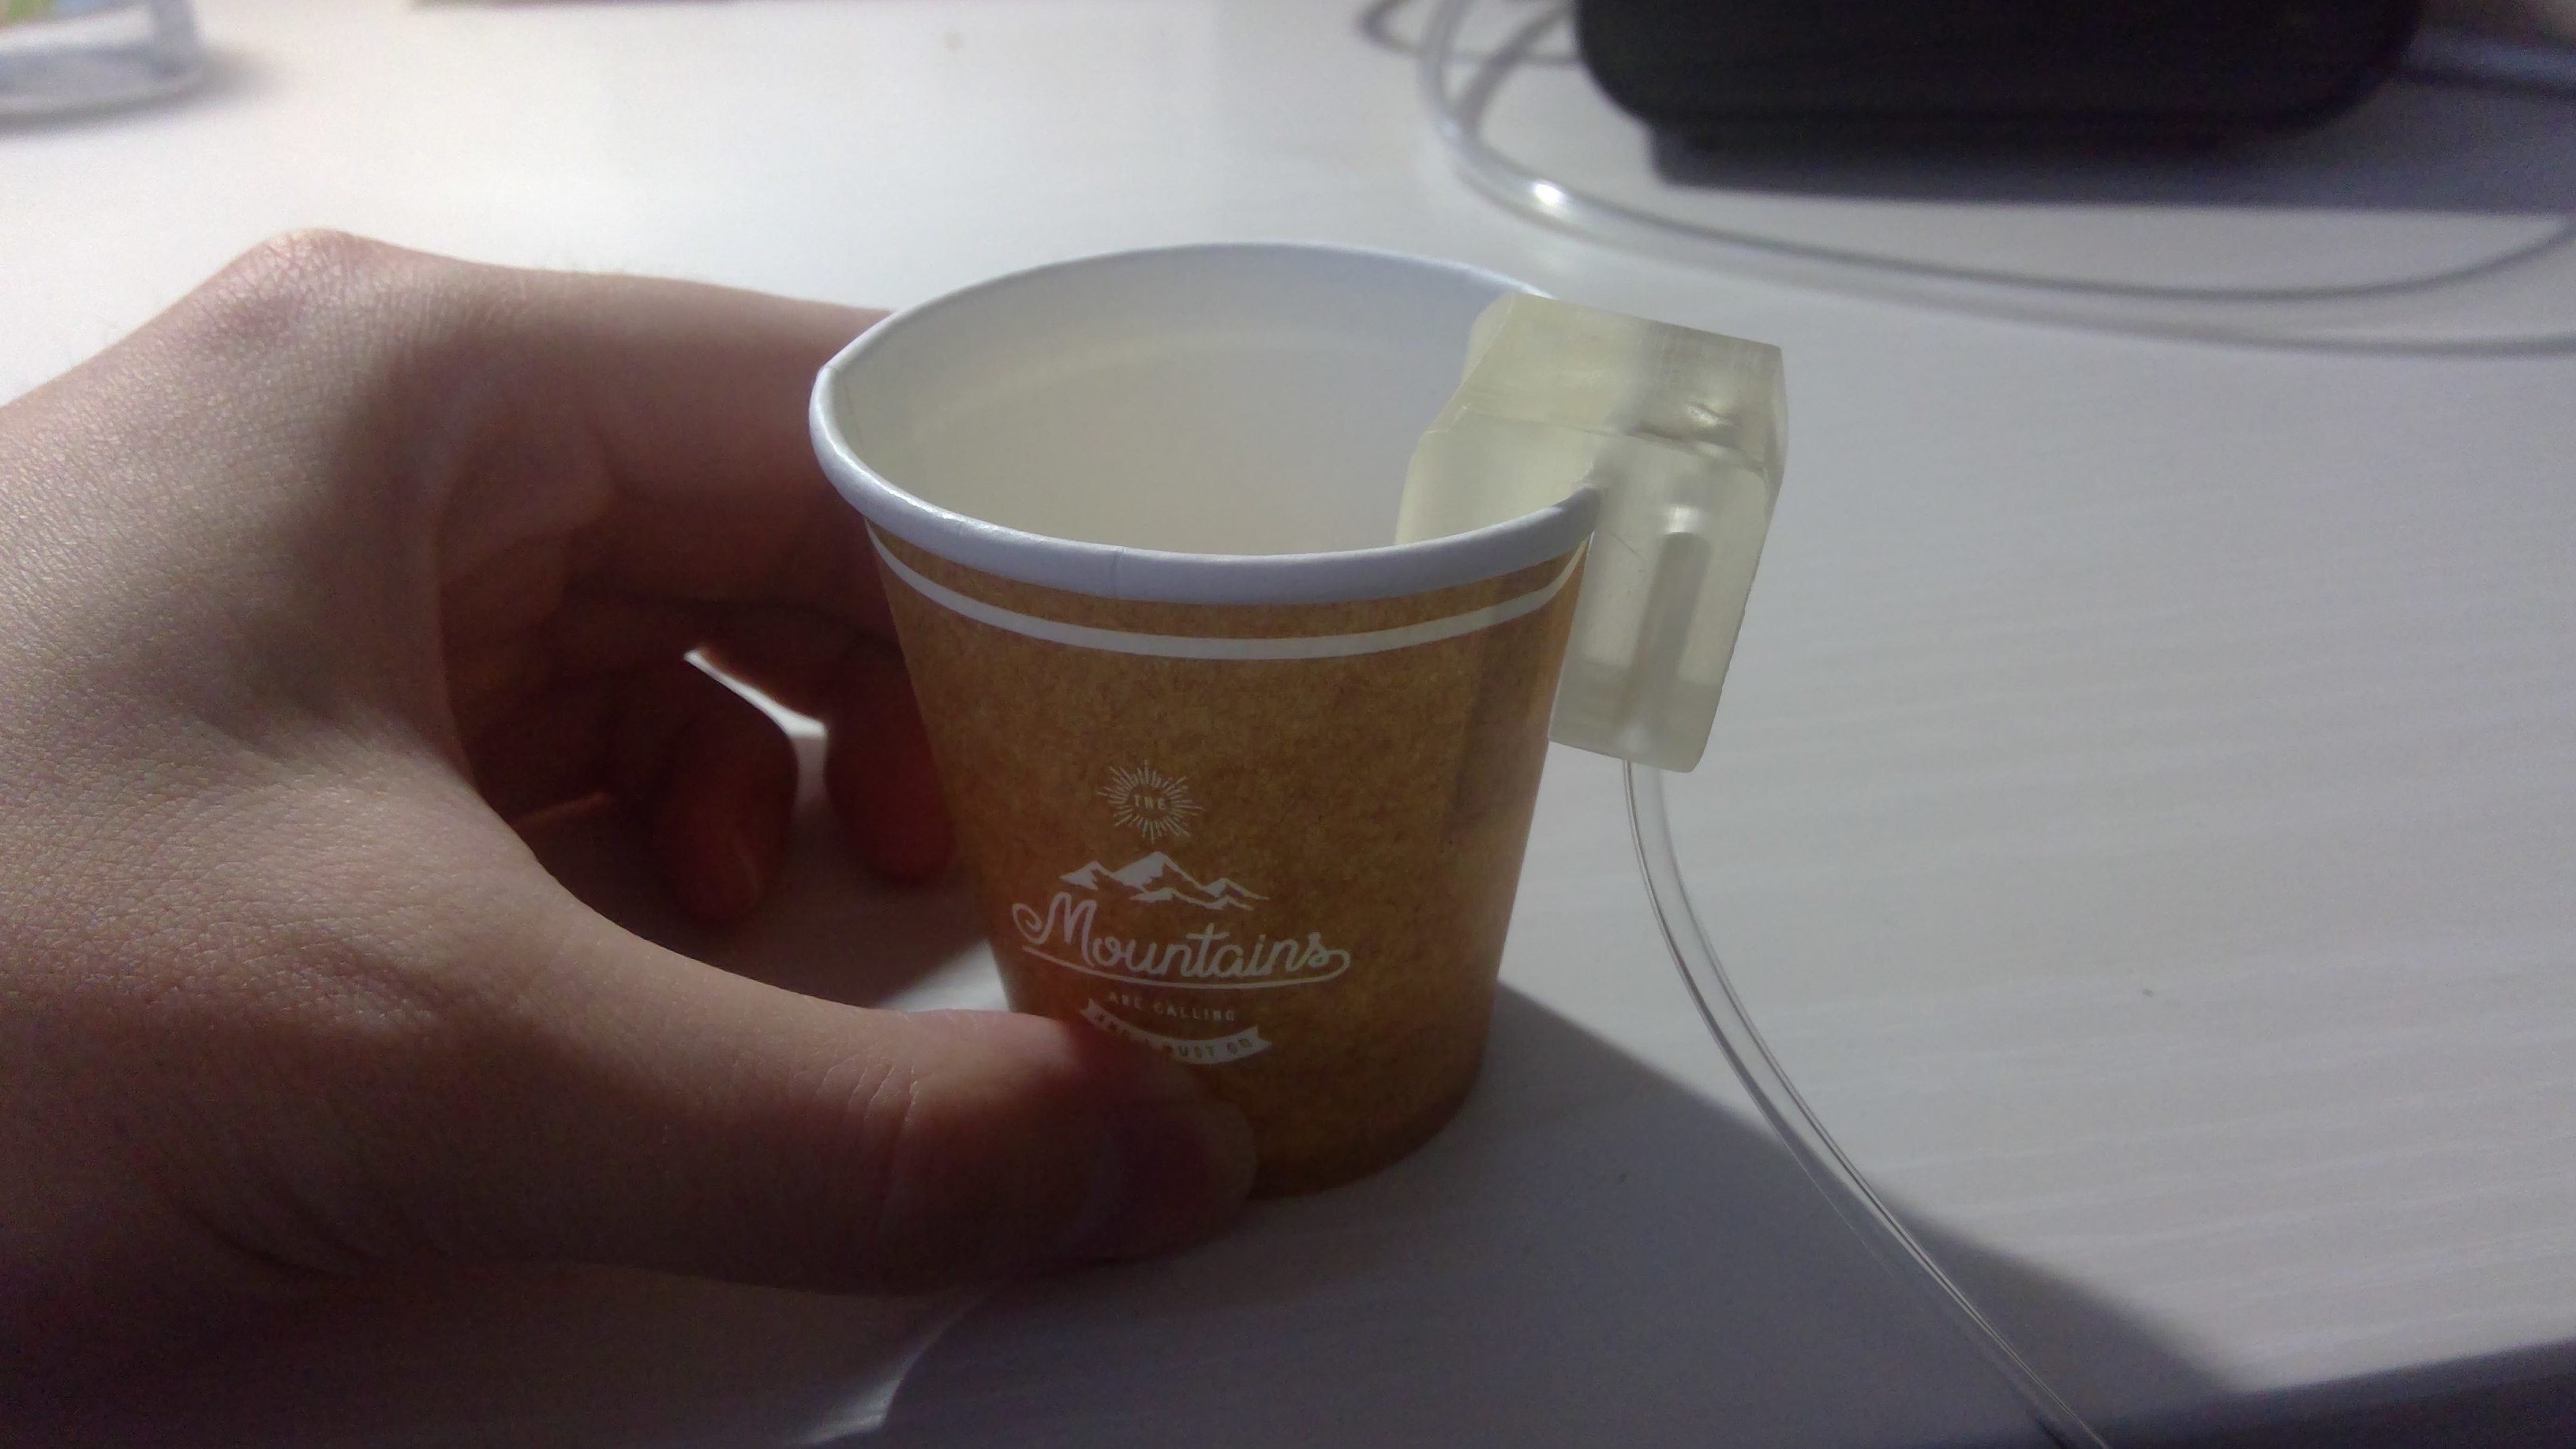
\includegraphics[width = 1.0\columnwidth]{figs/cup.jpg}
 %\includegraphics[width = 0.47\columnwidth]{figs/supunbody.jpg}
  \caption{嗅覚情報提示装置の全景}
  \ecaption{Panoramic view of olfactory information presentation device}
  \label{all}
\end{figure}

\begin{figure}[t]
  %\includegraphics[width = 0.47\columnwidth]{front2.jpg}
  %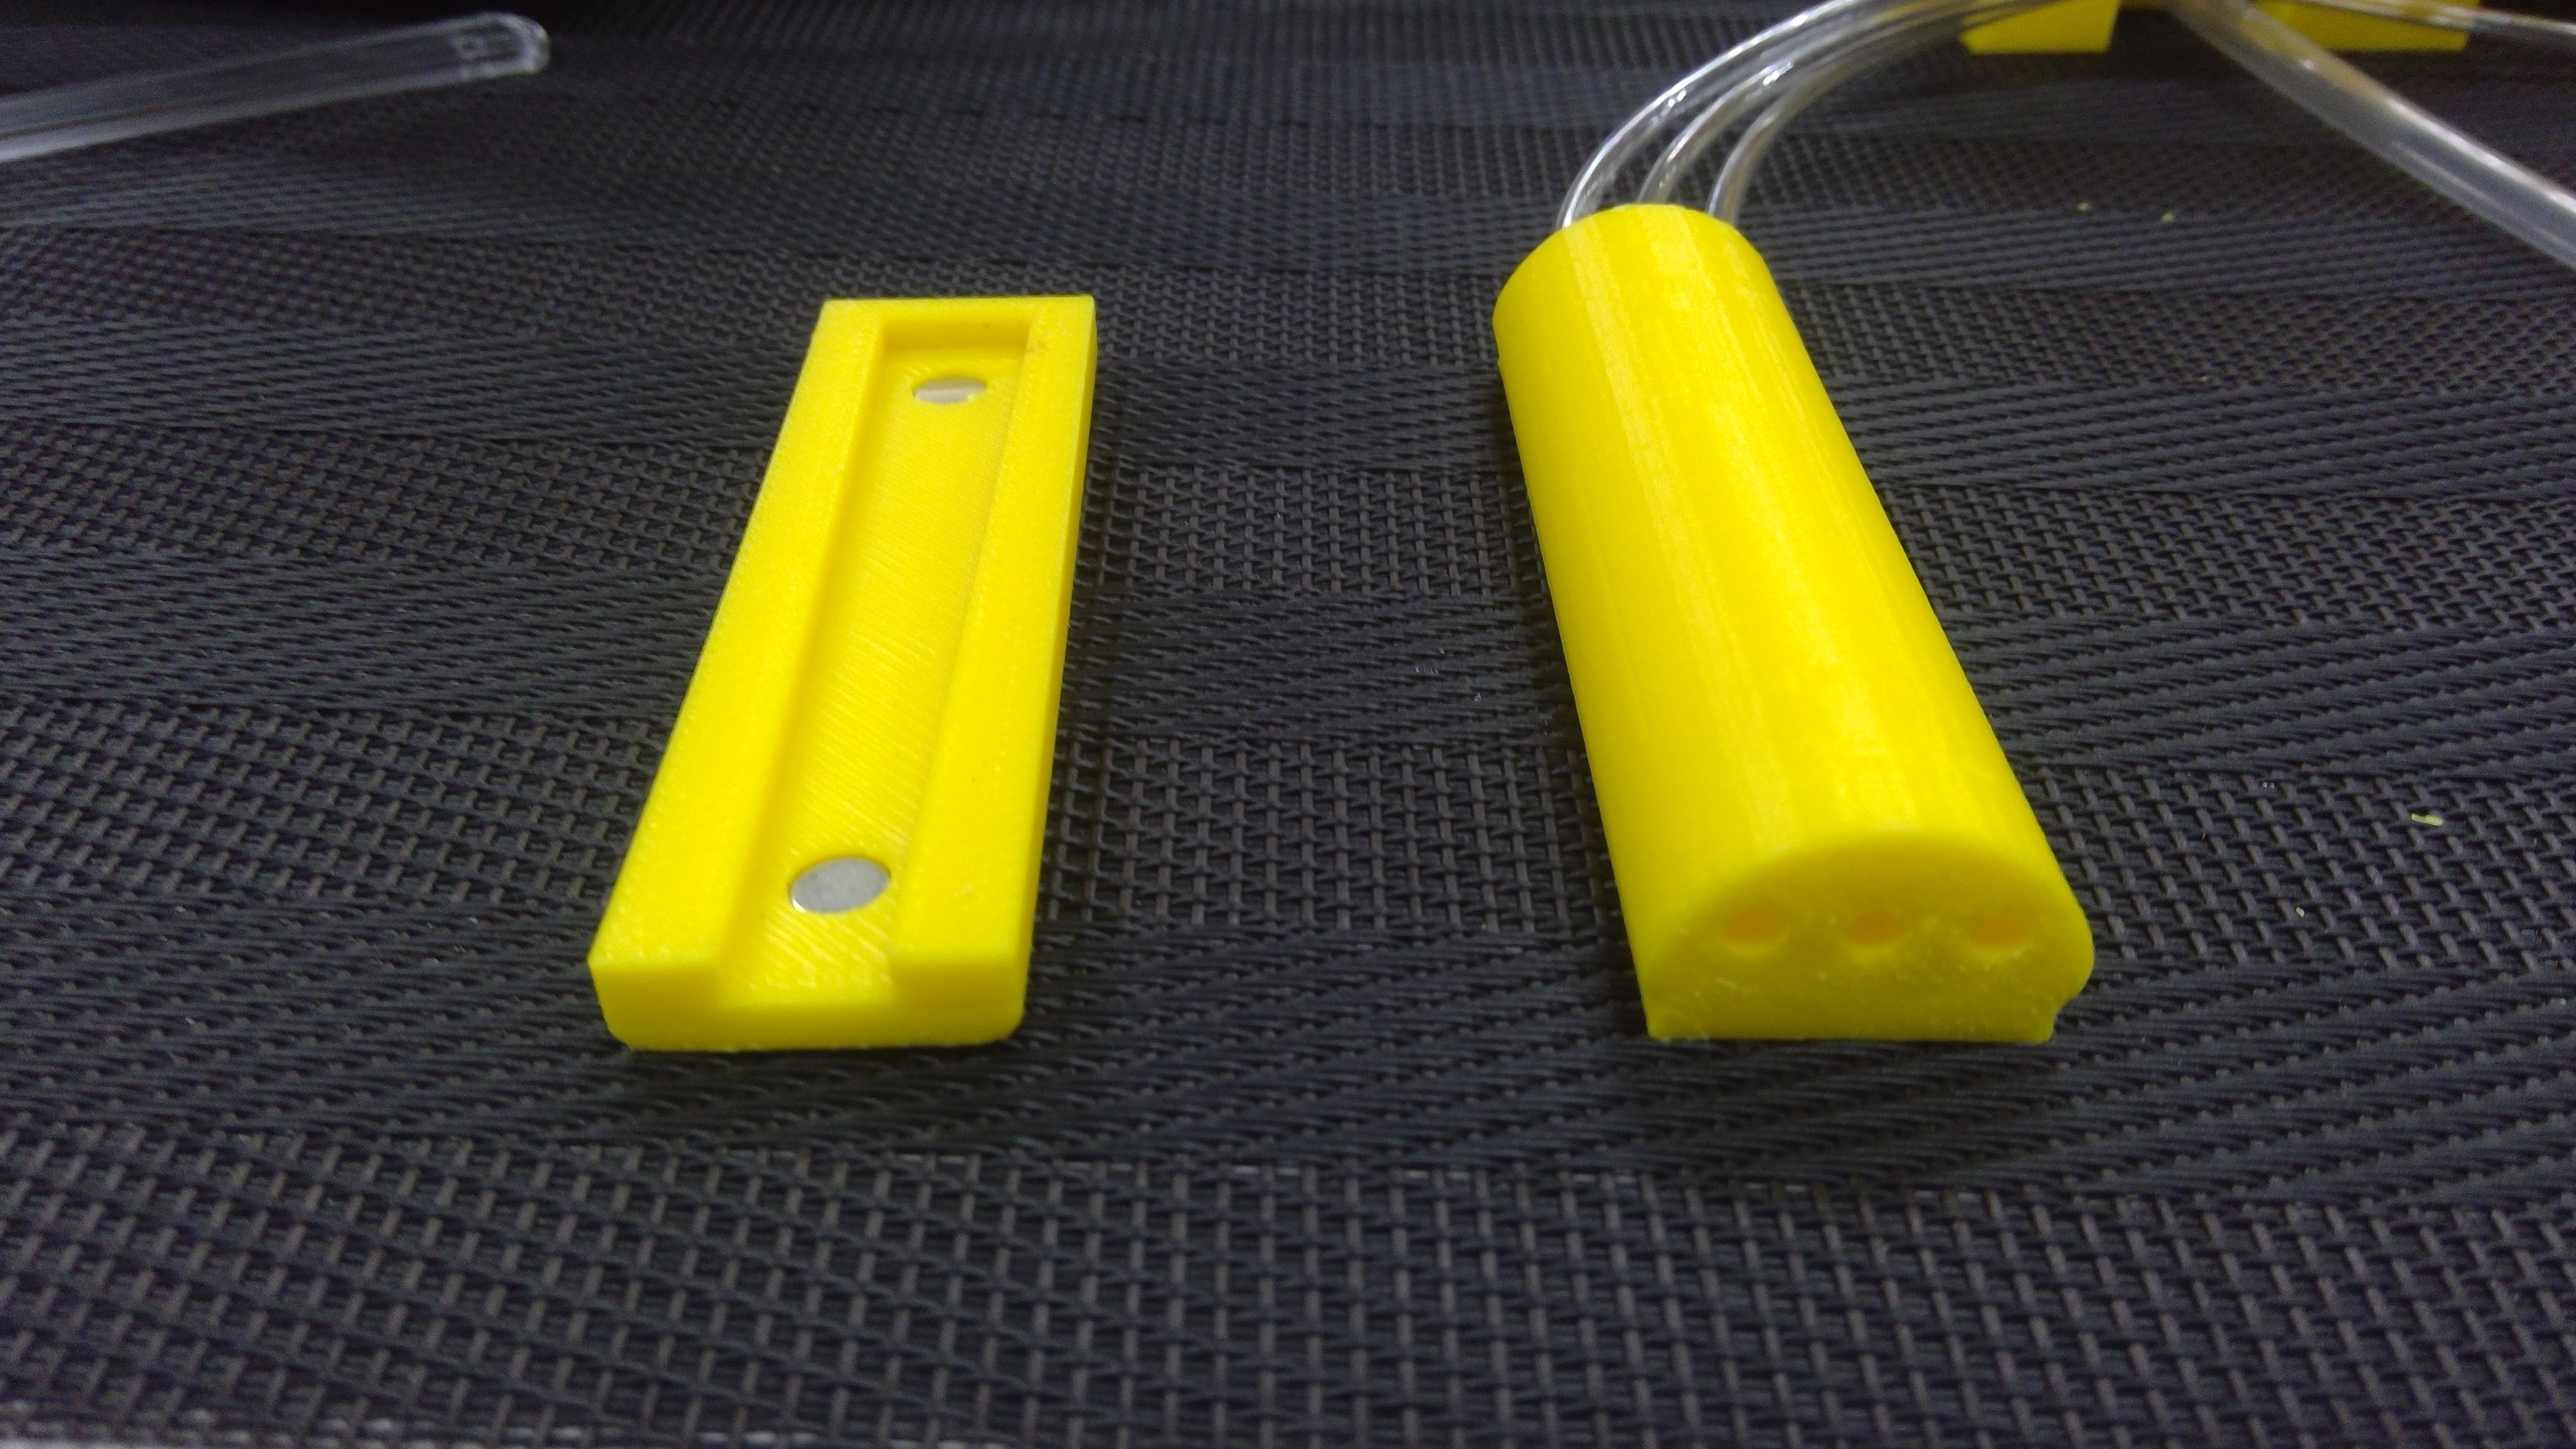
\includegraphics[width = 1.0\columnwidth]{supunpart.jpg}
  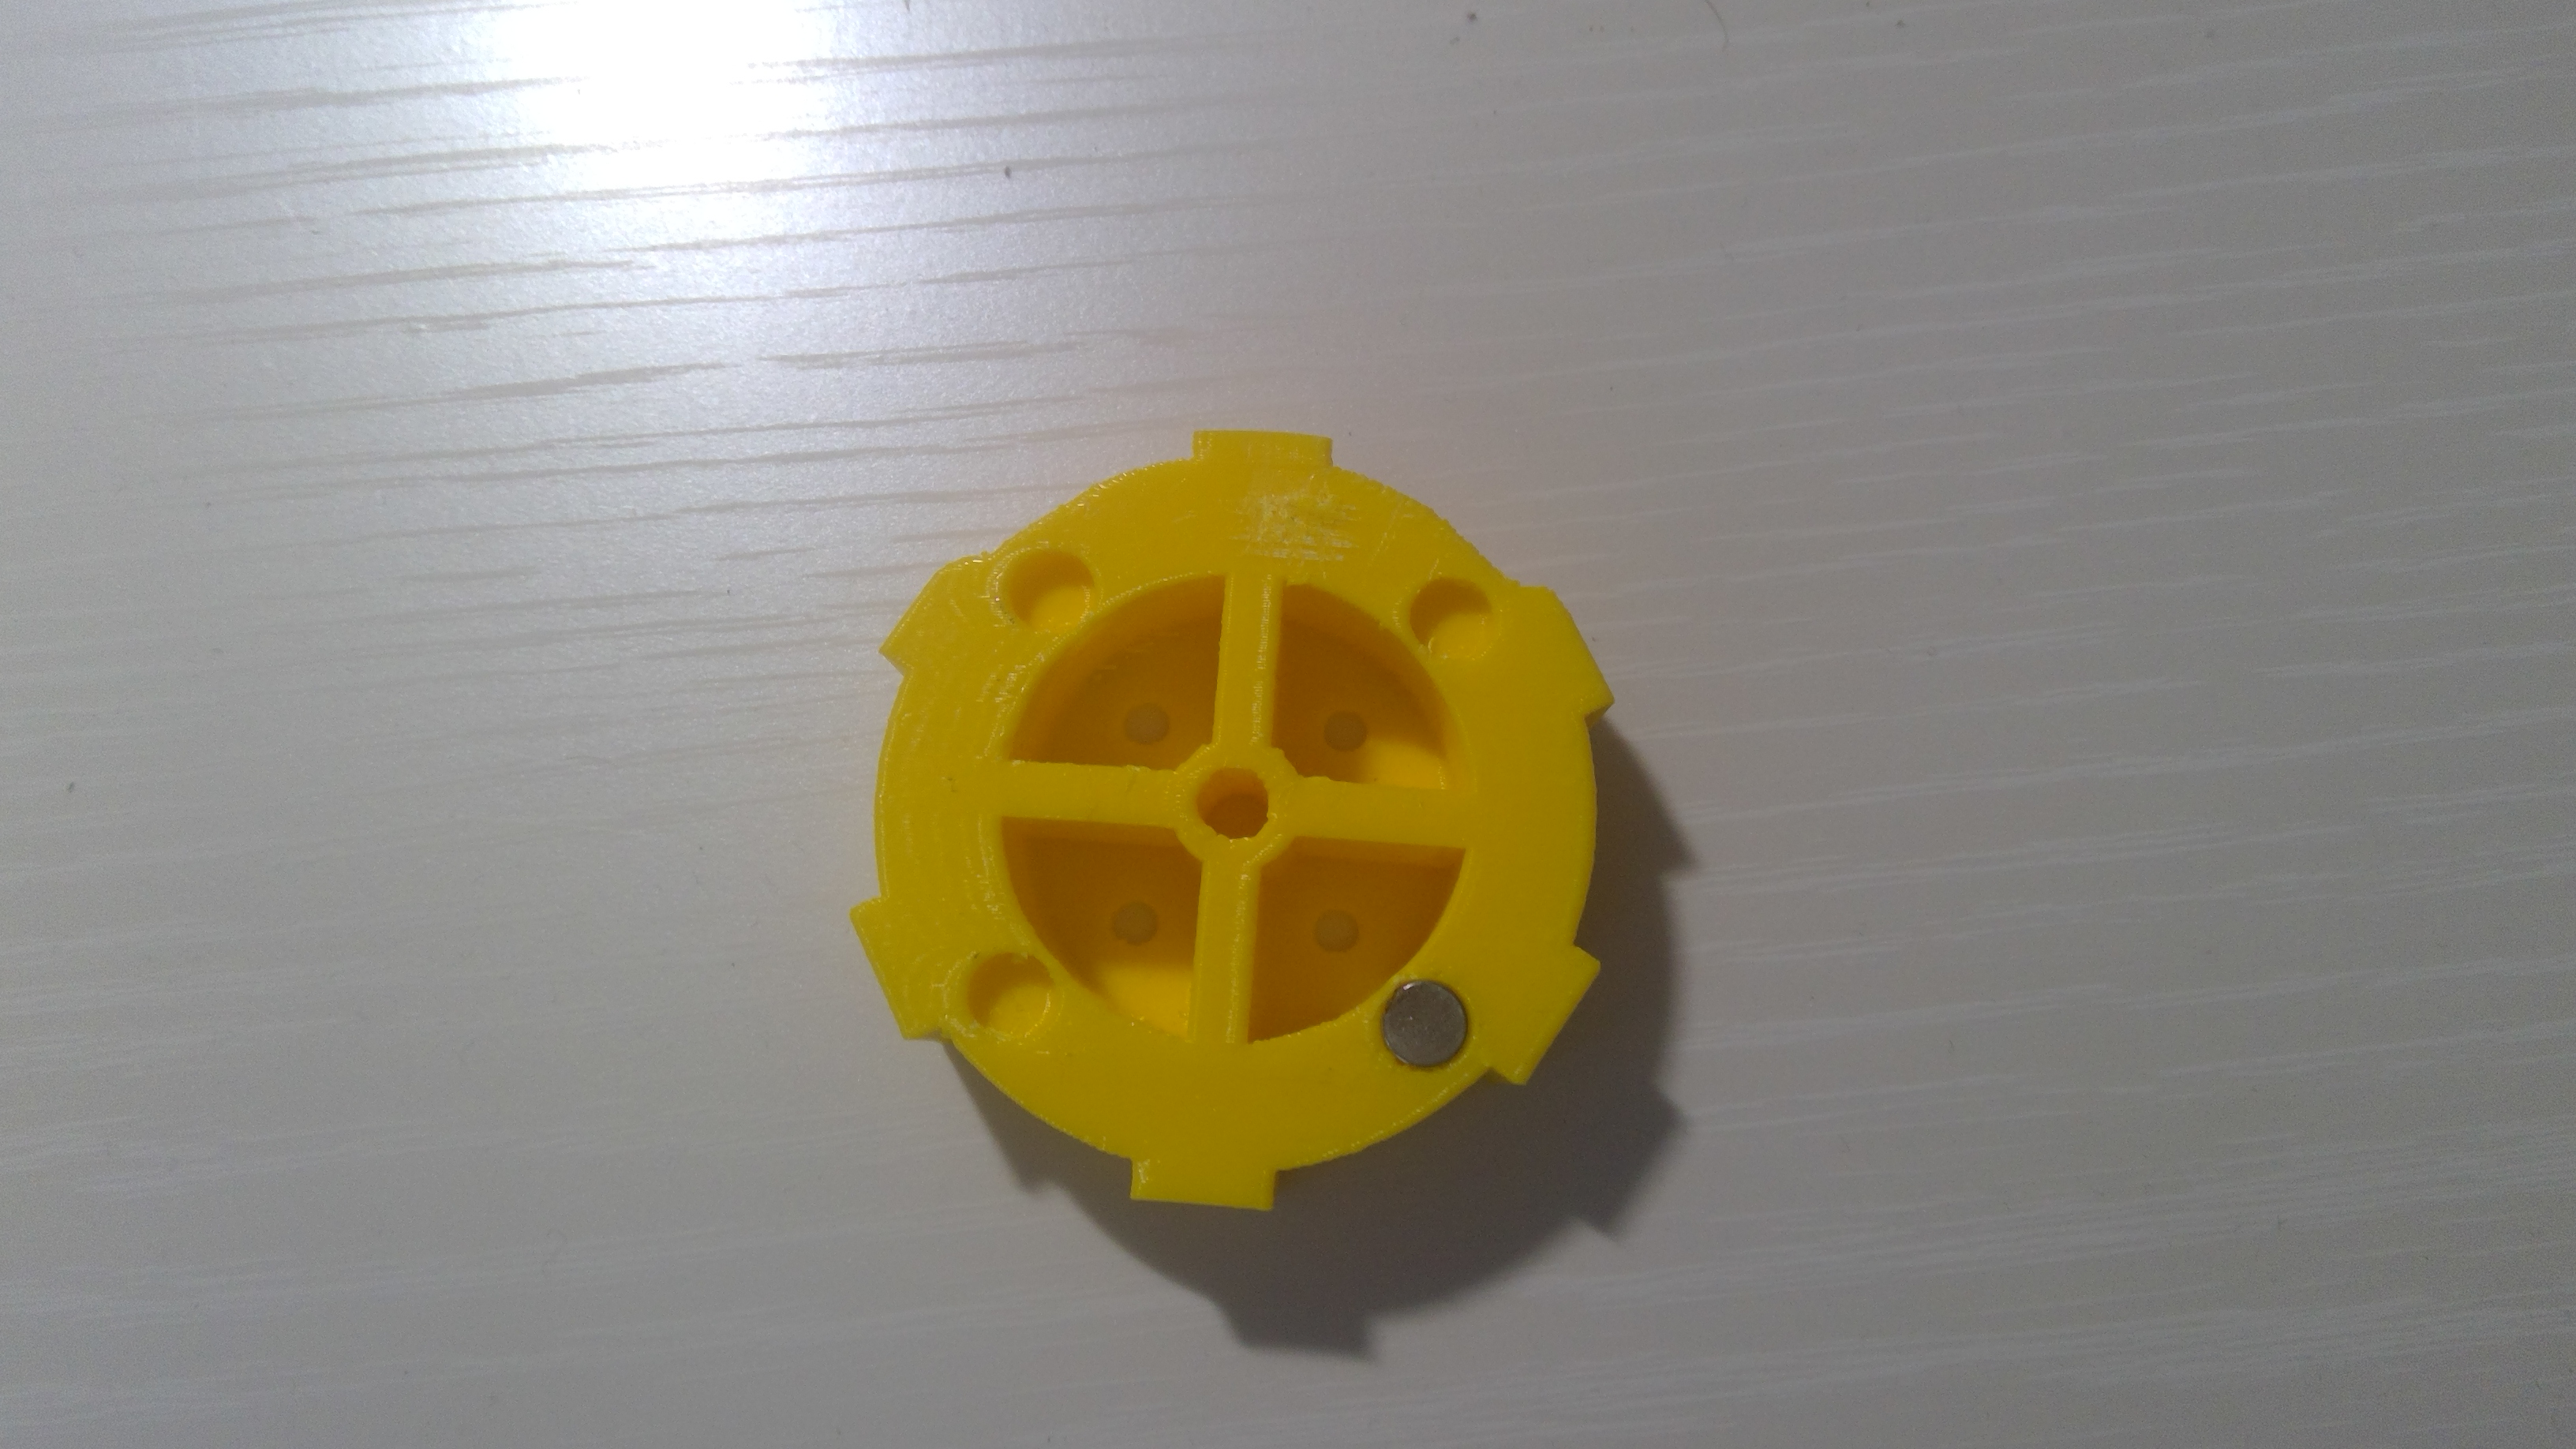
\includegraphics[width = 1.0\columnwidth]{figs/dial.jpg}
  \caption{香料切り替えデバイス}
  \ecaption{Spoon device}
  \label{device}
\end{figure}

使用する塩味スープを再現する香料の代わりとして,醤油・味噌の2種類の香りを外部刺激として使用する.
この二つは一般的に調味料としてしょっぱい味として認知されているものを選択した.




%本研究の目的は,嗅覚が与える影響を考慮し,それに視覚情報を加えることで,味覚に対しての認識を変化させることである.
%着色料を使用した色付けと食用の香料を含んだシロップで味わうかき氷においても視覚と嗅覚の違いで味に対する影響をもたらす.
%そのことから別の外部刺激で視覚と嗅覚にアプローチすることにより,通常のかき氷を同じような変化を再現することができるのではないかと仮説をたて検証した.
%そのために着色料を使用した色付けと食用の香料の代替品を用意し,嗅覚情報と視覚情報を提示するためのシステムを構築した.
%嗅覚面については香料の代わりとしてアロマオイル等の香りをファンを使用して鼻に伝達する.
%視覚面については着色料の代わりにLED光源を用いて色をつける.
%これら二つを組み合わせることで味覚変容を検討している.

%4
%% 3章 システムの構成
\section{味覚変容システム}
視覚情報と嗅覚情報を重畳する仕組みとして,LEDとエアポンプを用いたかき氷の味を変化させるためのシステムを試作している.
着色料や香料を用いると氷に混ぜ合わせる必要があり,1回ごとにかき氷を作り直す必要がある.そこでLEDを使用することで,その場での色の切り替えを可能とし.エアポンプを使用することで,手元で簡易に香りを送ることを可能とする.

これらによってリアルタイムに体験を行うことができるシステムを構築している.
本章ではこのシステムについての詳細を述べていく.

\subsection{システム概要}
本システムは,視覚情報を提示する部分と,嗅覚情報を提示する部分の二つで構成されるシステムである.
かき氷の容器としてショットグラスにLEDを当てるシステムを組み込み,かき氷を食べる際には嗅覚情報が提示されるデバイスをスプーンに取り付ける.
これらのシステムはWi-fiやBluetoothを内蔵したマイコンである「ESP32」と「Arduino」に書き込んだプログラムによって制御を行う.
以下では二つの構成要素についての詳細を述べていく.
%3.3 視覚
\subsection{視覚情報提示}
\begin{figure}[t]
  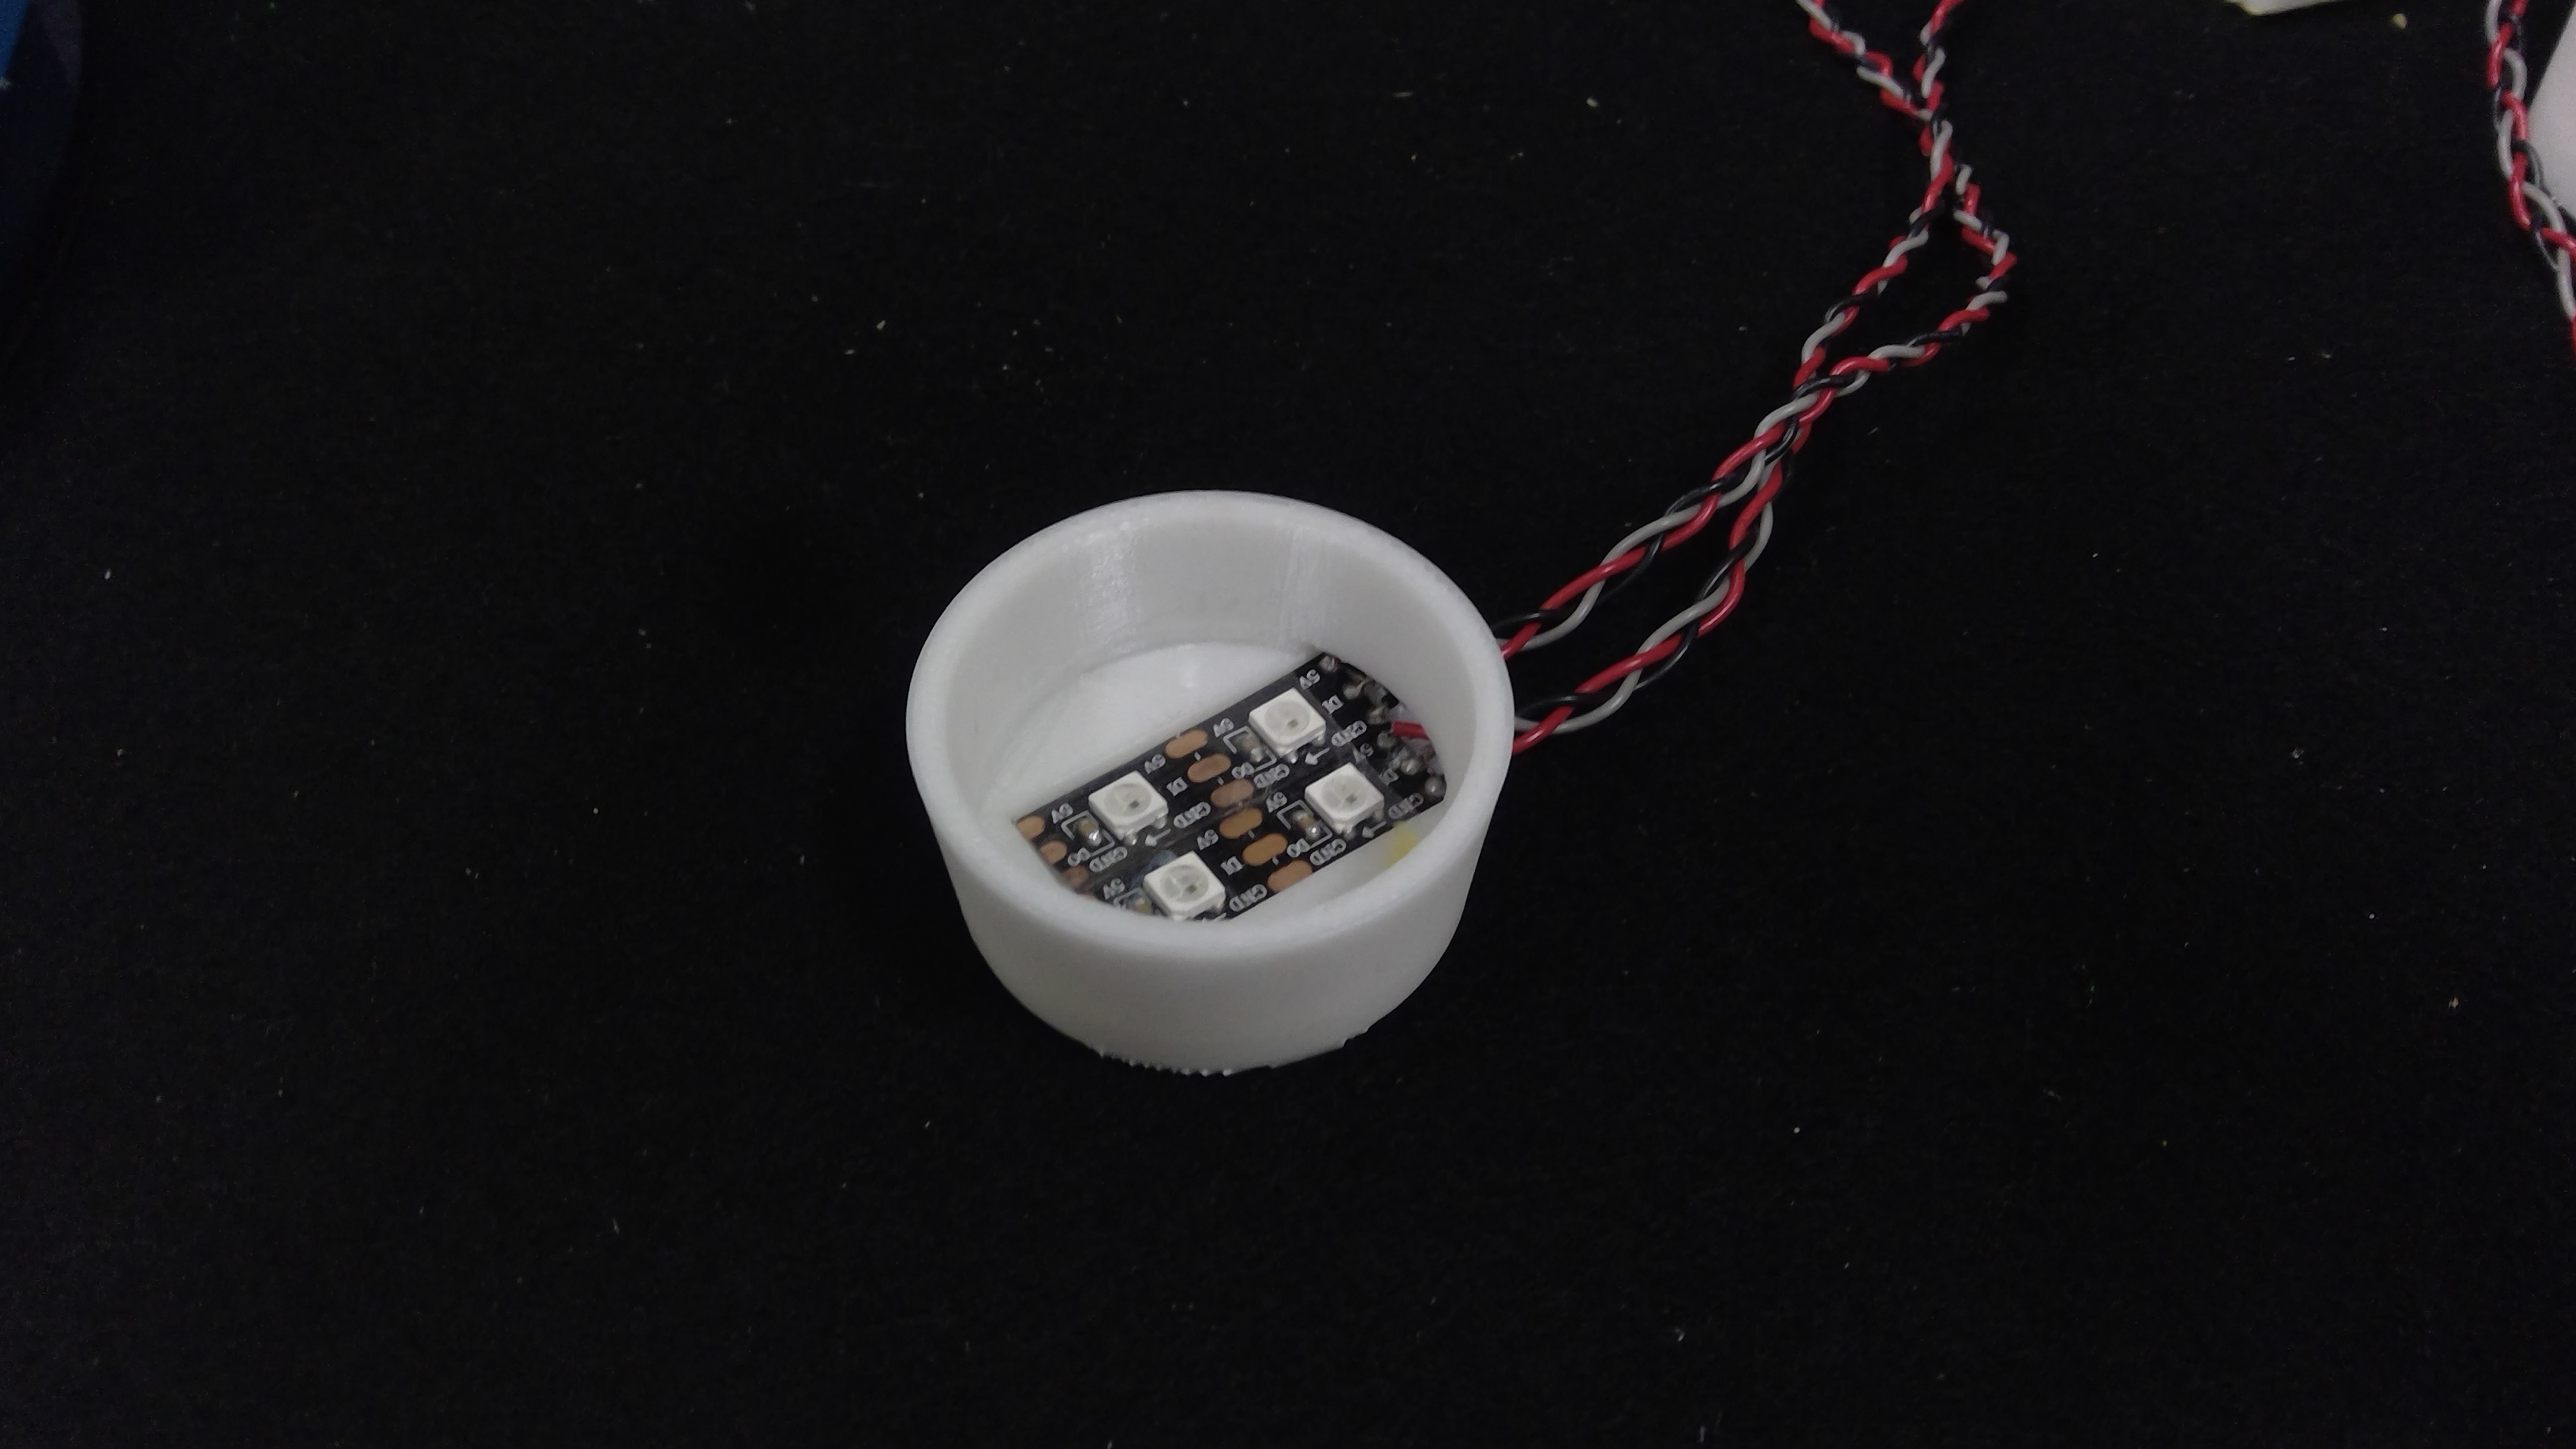
\includegraphics[scale = 0.075]{figs/coaster.jpg}
  \caption{LEDコースタ―}
  \label{coaster}
\end{figure}
\begin{figure}[t]
  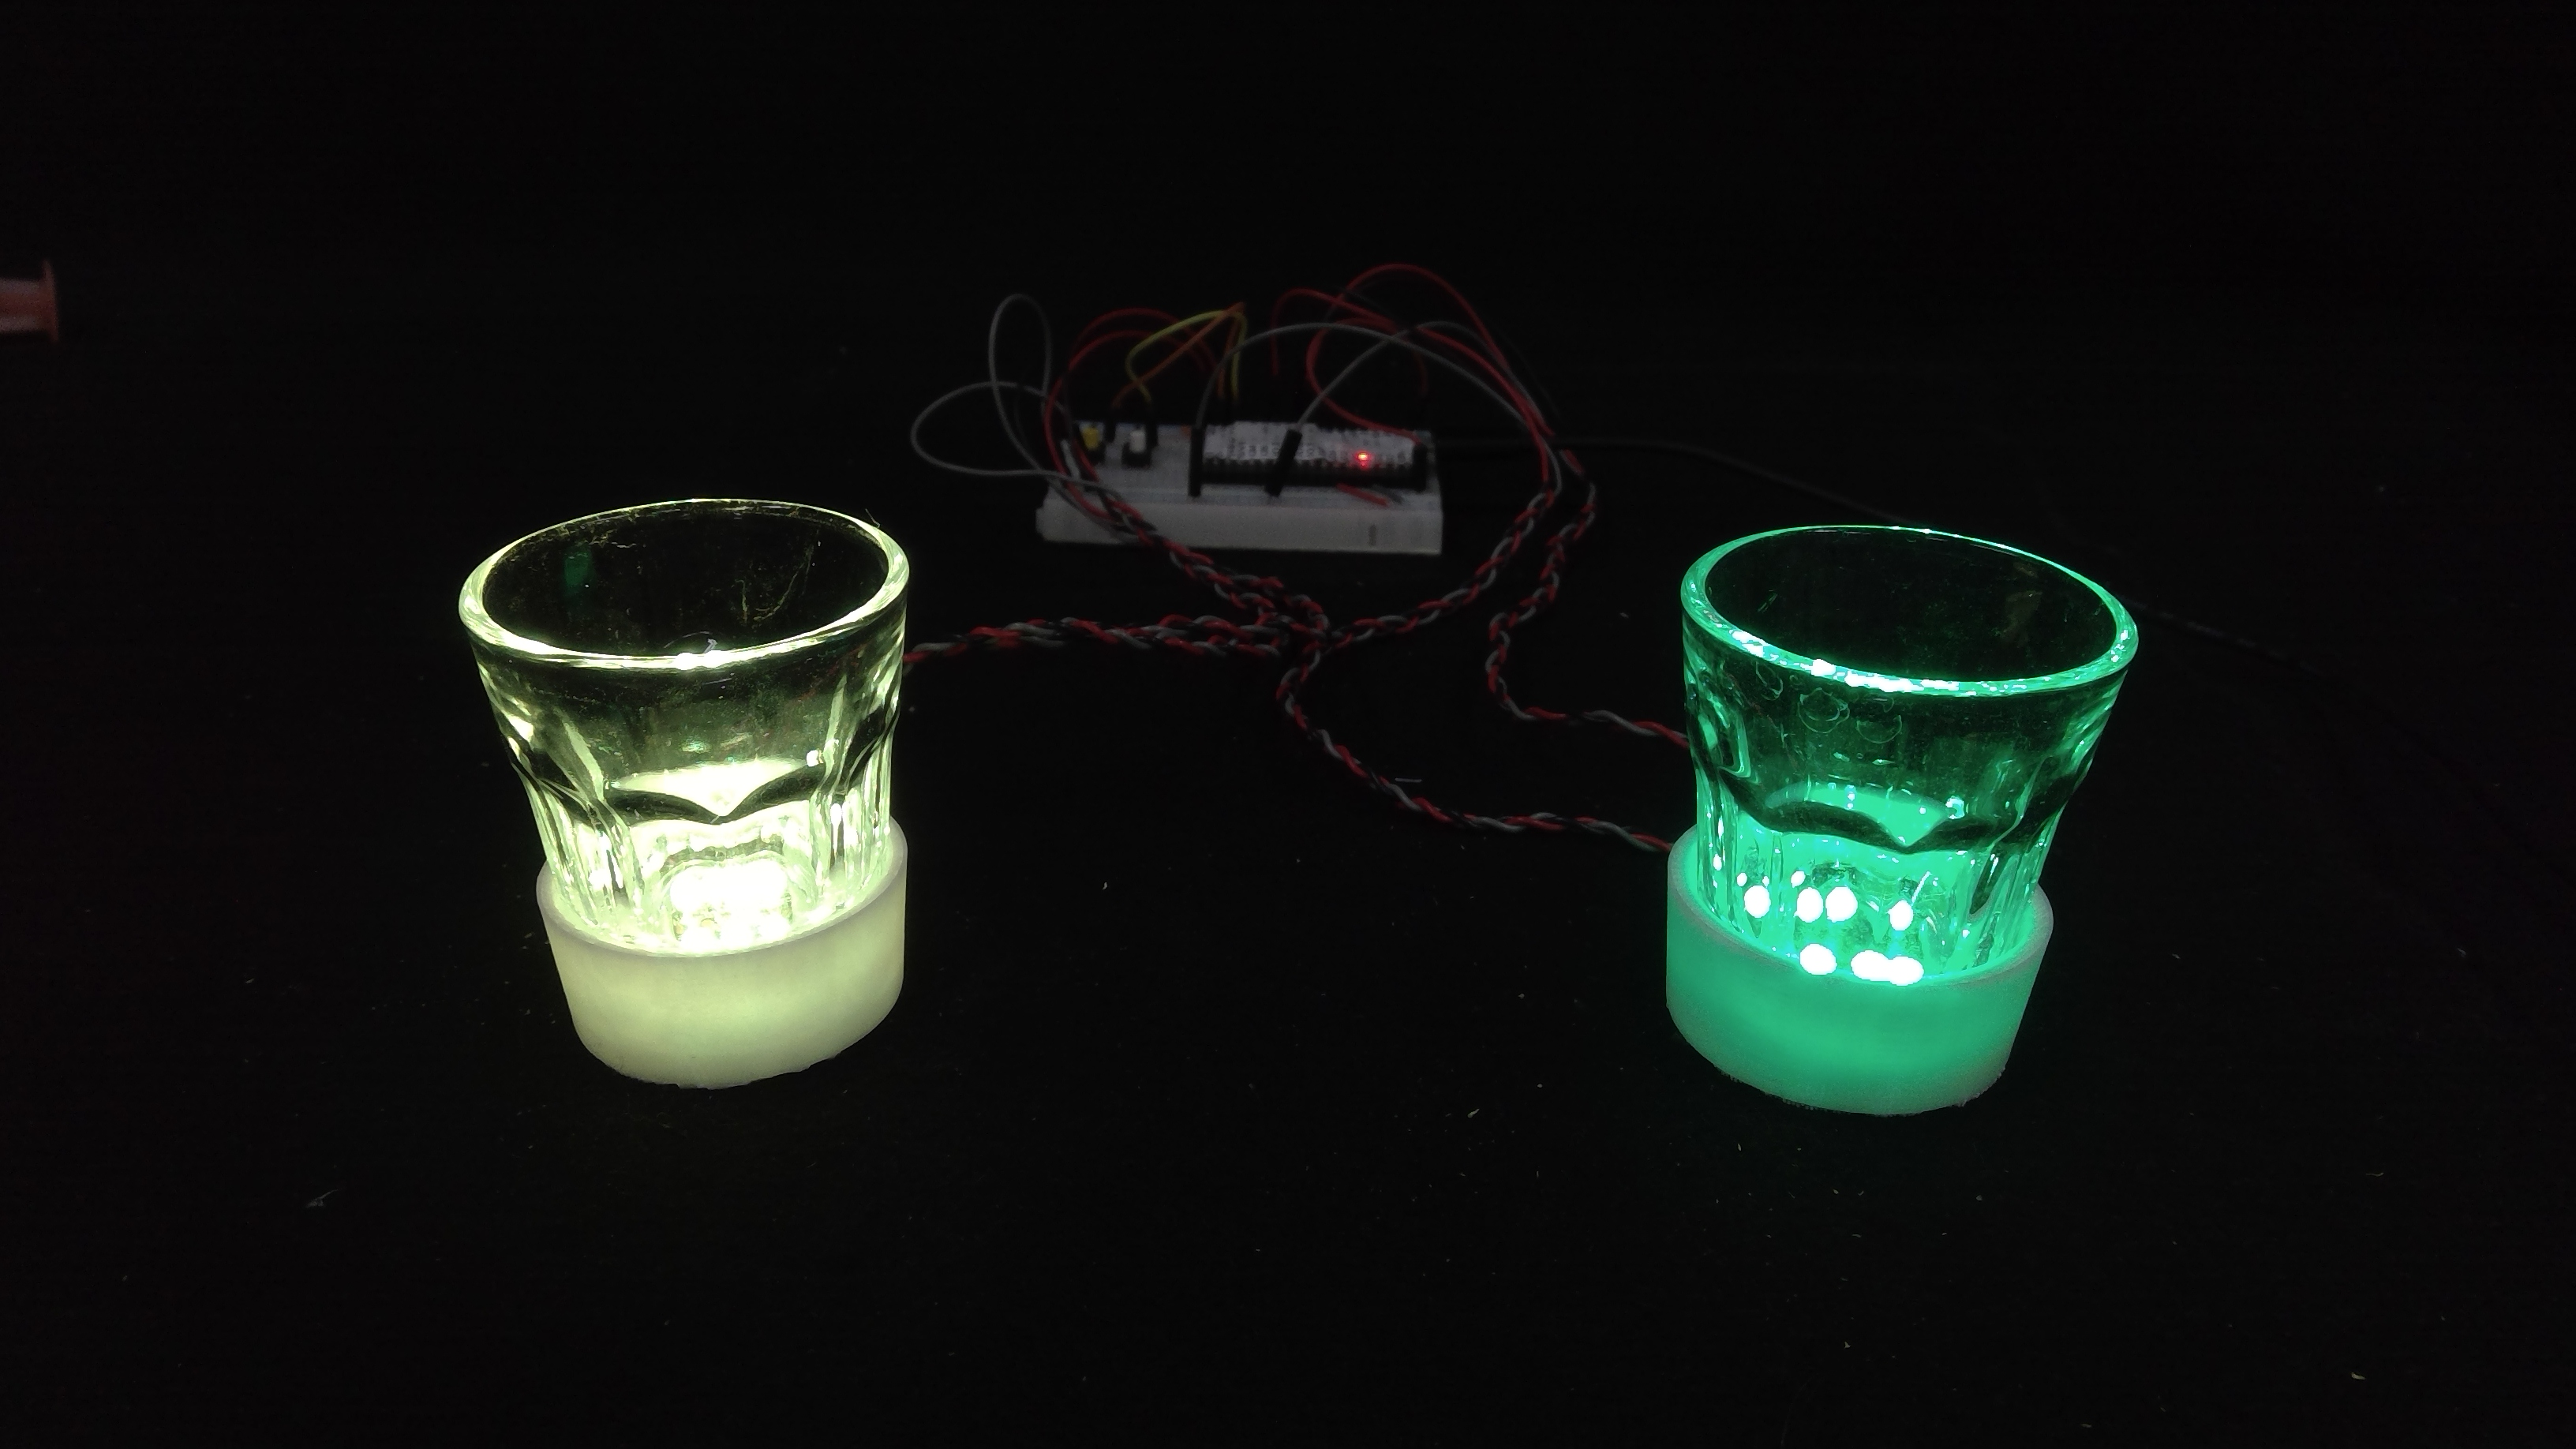
\includegraphics[scale = 0.075]{figs/gluss.jpg}
  \caption{LEDで照らされたショットグラス(黄色・緑色)}
  \label{gluss}
\end{figure}


かき氷におけるシロップの色の再現については,着色料の代わりとしてフルカラーのLEDを使用した.
LEDテープを透明なショットグラスの裏に設置するために図\ref{coaster}のようなコースターを作成した.
LEDの上面は透明なテープで覆うことで,ショットグラスから垂れる水滴が入らないようにしている.
このコースターを使用することで図\ref{gluss}のように,かき氷自体を照らすことが可能になり,また容器を持ち上げることができ,食べる瞬間まで色を感じることができる.
LEDの制御として,その場での切り替えをするためにタクトスイッチを用意し,それによって点灯または消灯の制御を行っている.
通常のかき氷では,削られた氷の上面にシロップの色がついているものだが,今回は色の印象強く与えることによる錯覚を重視し,かき氷全体に色を付けることとした.

%色がついているという印象を強く与えることを優先したために,この手法を採用することとした.
この手法を用いると,LEDの熱で氷が解けることが懸念されるため検証を行った.部屋の気温を22度で設定し,LEDコースターで照らされたかき氷は,4分以上はある程度の形を保ったままであった.そのため,実験の際には支障がないと判断した.

%\begin{figurfee}
%  \includegraphics[width = 0.32\columnwidth]{ice.jpg}
%  \includegraphics[width = 0.32\columnwidth]{ice2.jpg}
%  \includegraphics[width = 0.33\columnwidth]{ice3.jpg}
%  \caption{スプーン側のLED
%  (無色・黄色・白色)}
%  \label{ice}
%\end{figure}

LEDを使用する理由として,色の切り替えをスムーズに行えるという点が挙げられる.近年では見た目を変える手法としてはVRを使った手法がたくさん行われているが,可用性に欠けたり,食べ辛かったりする.そこでデバイスを渡すだけで簡単に行えることや現実的な視覚としての実験を行うことに意味があると考えた.また,関連研究にも挙げた「LED光源を用いて色を重畳した場合にも,着色料を用いて色を付けた際と同程度のクロスモダリティ効果があった」という実験結果を踏まえても,この手法は有意義であると考える.

色の選択として,使用する2種類の香りの印象の強い色を使用しショットグラスの容器を照らした.レモンの色を黄色,メロンの色は緑色とした.

\subsection{嗅覚情報提示}
香りを嗅がせる方法として,図\ref{all}の嗅覚情報提示装置を製作した.
香りを送るための仕組みを含んだボディやケースを3Dプリンタで作成している.
全体の流れの構成を図\ref{flow}に示す.エアポンプから配送された風はチューブを通り,制御されたエアー分岐管を通ることで3つの経路に分かれる.2つの経路では,香りを含ませた脱脂綿を仕込んだ香り瓶の中を経由して香料を付与した風となり,残りの一つは何も含まない風となる.この3つをまとめたものがスプーンデバイスに組み込まれており,スプーンを口に運んだ際に,鼻に香りを付与した風が当たるものとなっている.


\begin{figure}[t]
  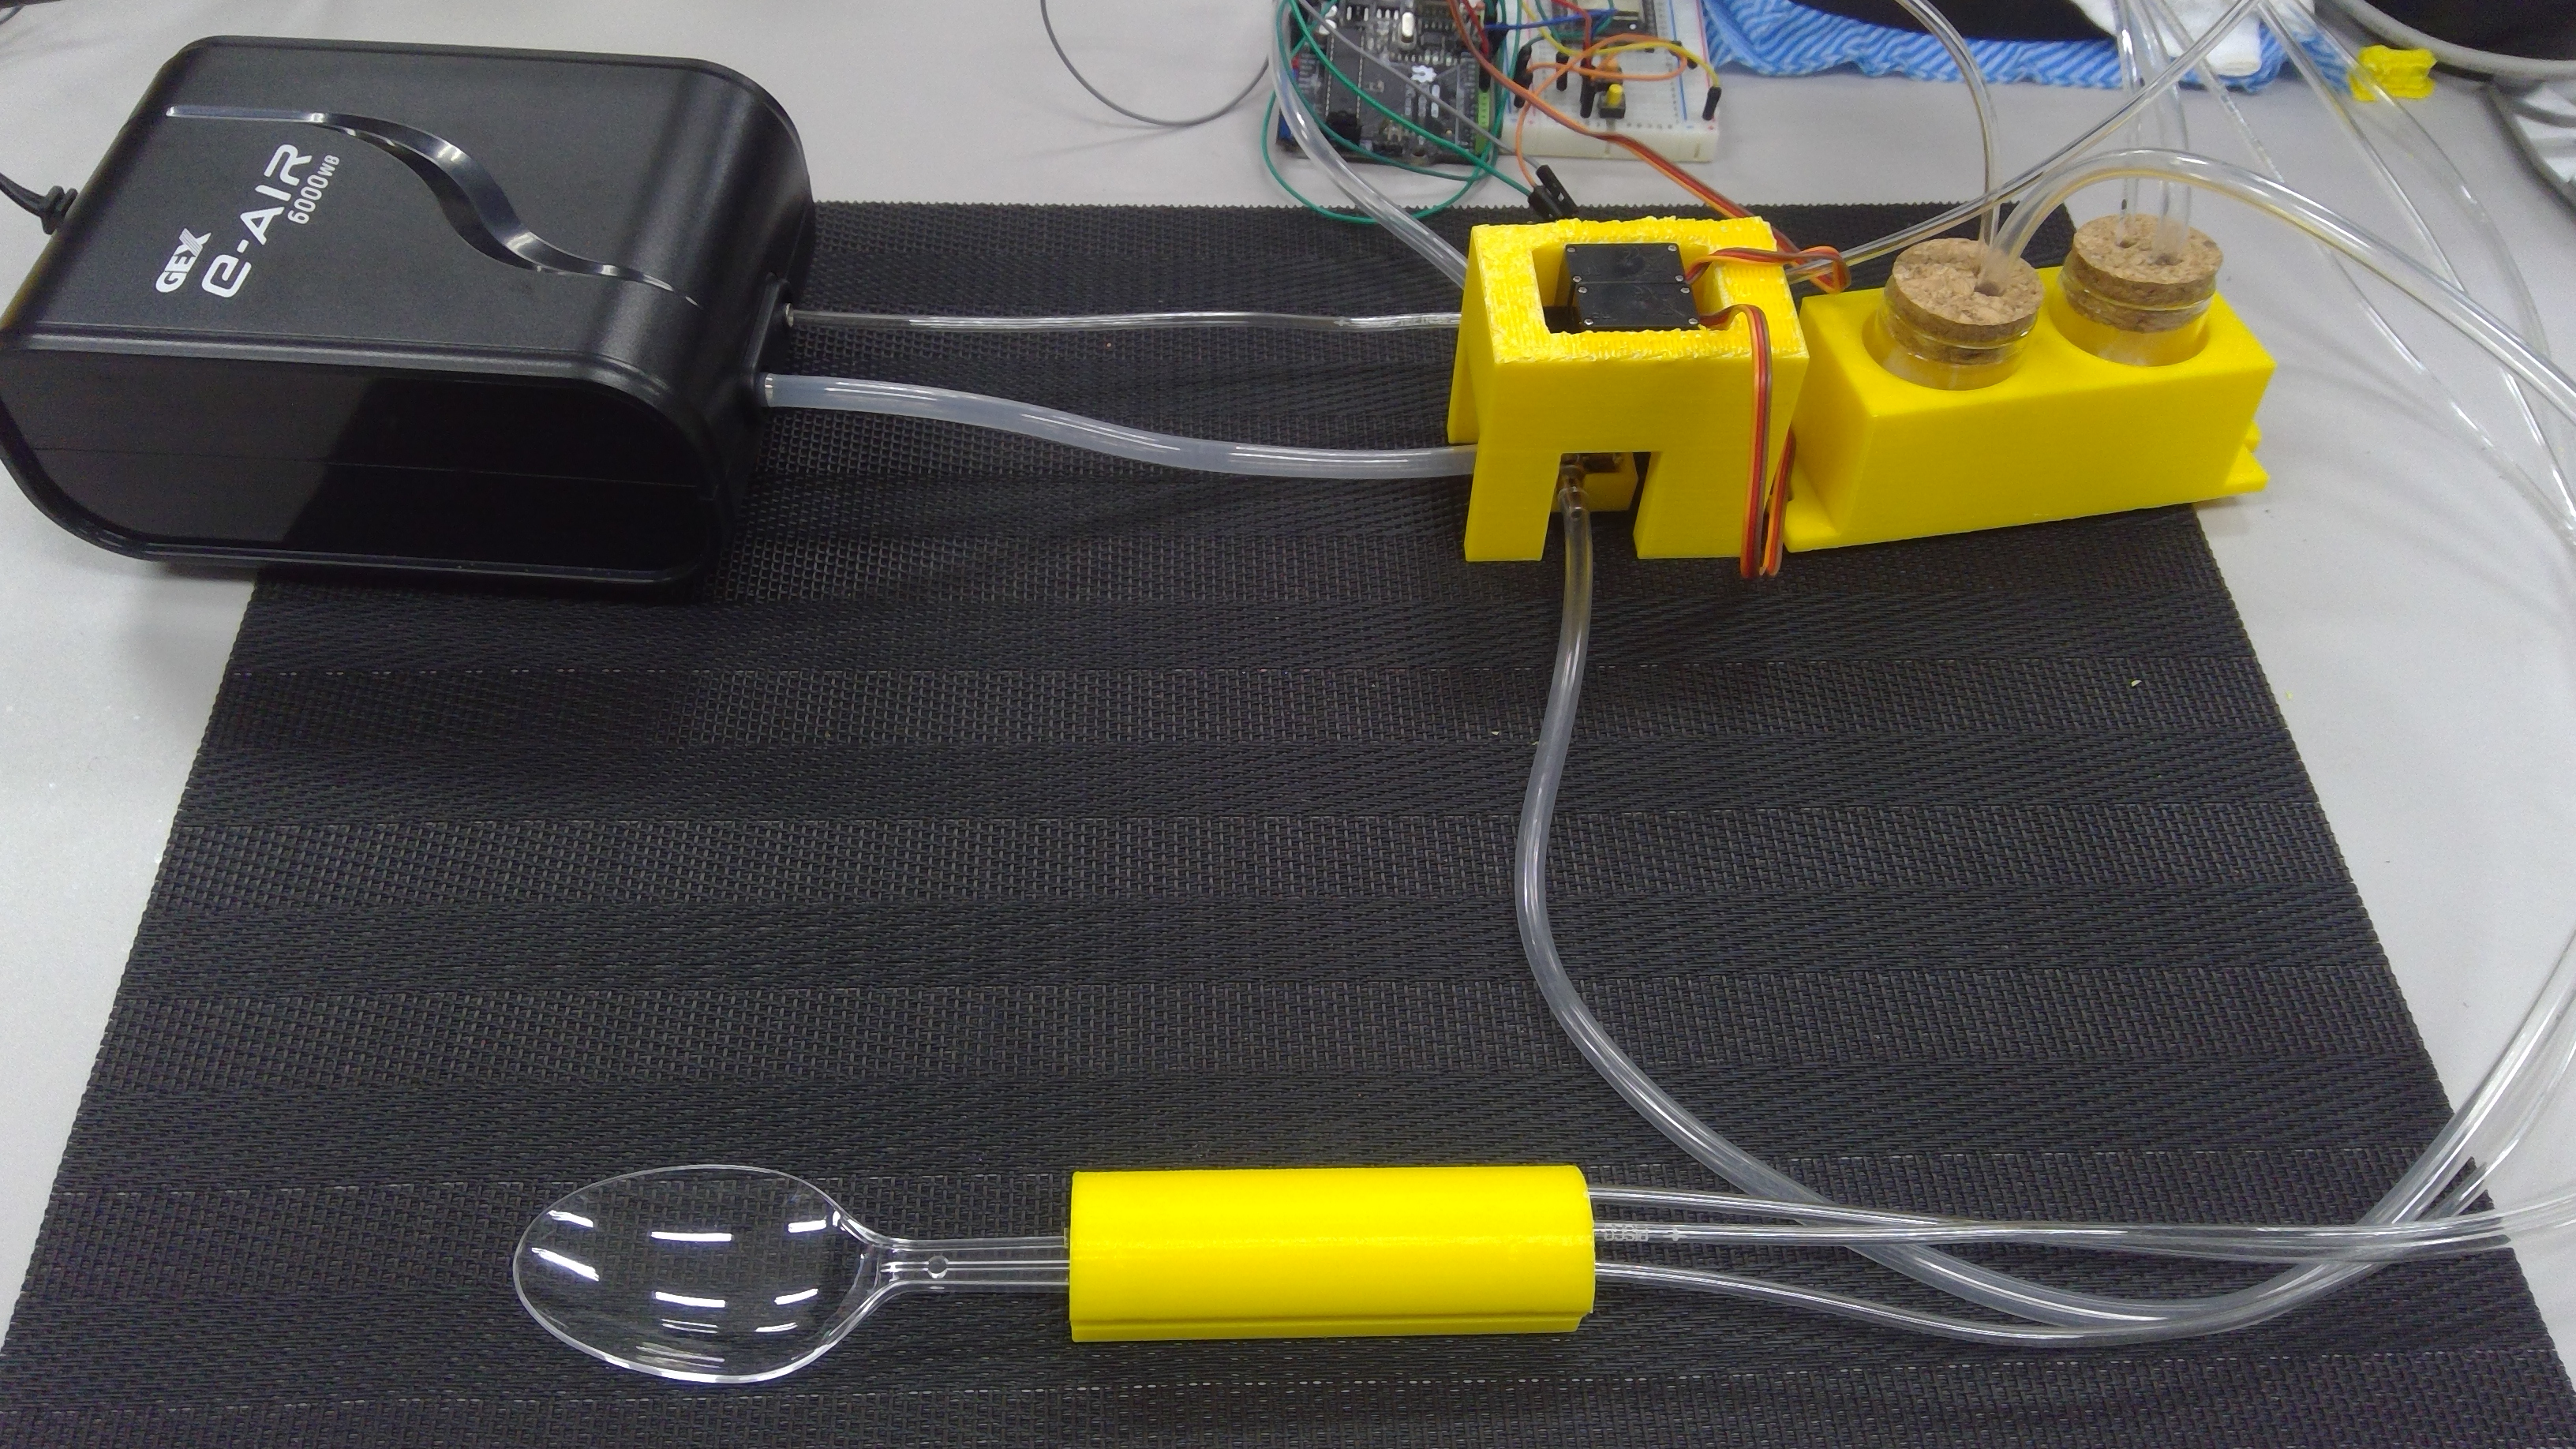
\includegraphics[width = 1.0\columnwidth]{all.jpg}
  \caption{嗅覚情報提示装置の全景}
  \label{all}
\end{figure}

\begin{figure}[t]
  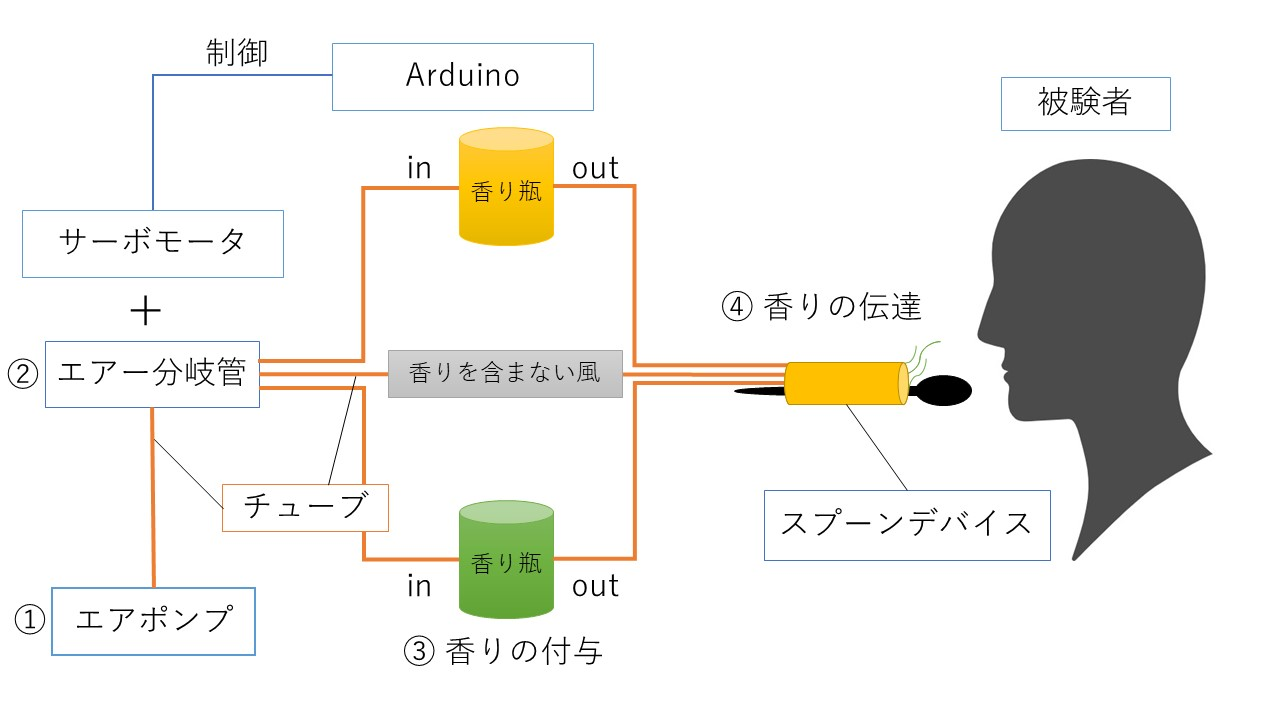
\includegraphics[width = 1.0\columnwidth]{flow.jpg}
  \caption{香り配送の流れ}
  \label{flow}
\end{figure}


\subsubsection{香料}
かき氷のシロップに含まれている香料の代わりとして,レモン・メロンの2種類の香りを外部刺激として使用する.

レモン・メロンは共に既存のシロップの味として存在しており,出店にもあるベーシックな味である.レモンは以前の研究から,有効性が確かめられており,デバイスが変わっても有効性を調査するために選んだ
.メロンの香りは新たな香りの検証として,甘味を感じやすい香りという点からも味の違いに差が出るのではないかと仮説を立て,選択した.

香りを感じさせる方法は,レモンはアロマオイル(天然植物精油)を使用し,メロンは市販の食品添加物から,それぞれ液体となっている香料を脱脂綿に染み込ませ,その香りを嗅がせることとした.この実験においてはレモンの味の再現としてレモンの香りではなくライムの香りを使用している.以前の研究の予備実験において,10人に対してどちらのほうがレモン味のかき氷の香りに近いかを尋ねたところ,ほとんどがライムの香りを選択している.ライムの香りのほうがレモン味のかき氷の風味に似ているという点から、今回もライムの香りを使用している.

\subsubsection{スプーンデバイス}
図\ref{device}に示したスプーンデバイスはスプーンとして持つ際に抵抗が出ないように作成している.
\begin{figure}[t]
  %\includegraphics[width = 0.47\columnwidth]{front2.jpg}
  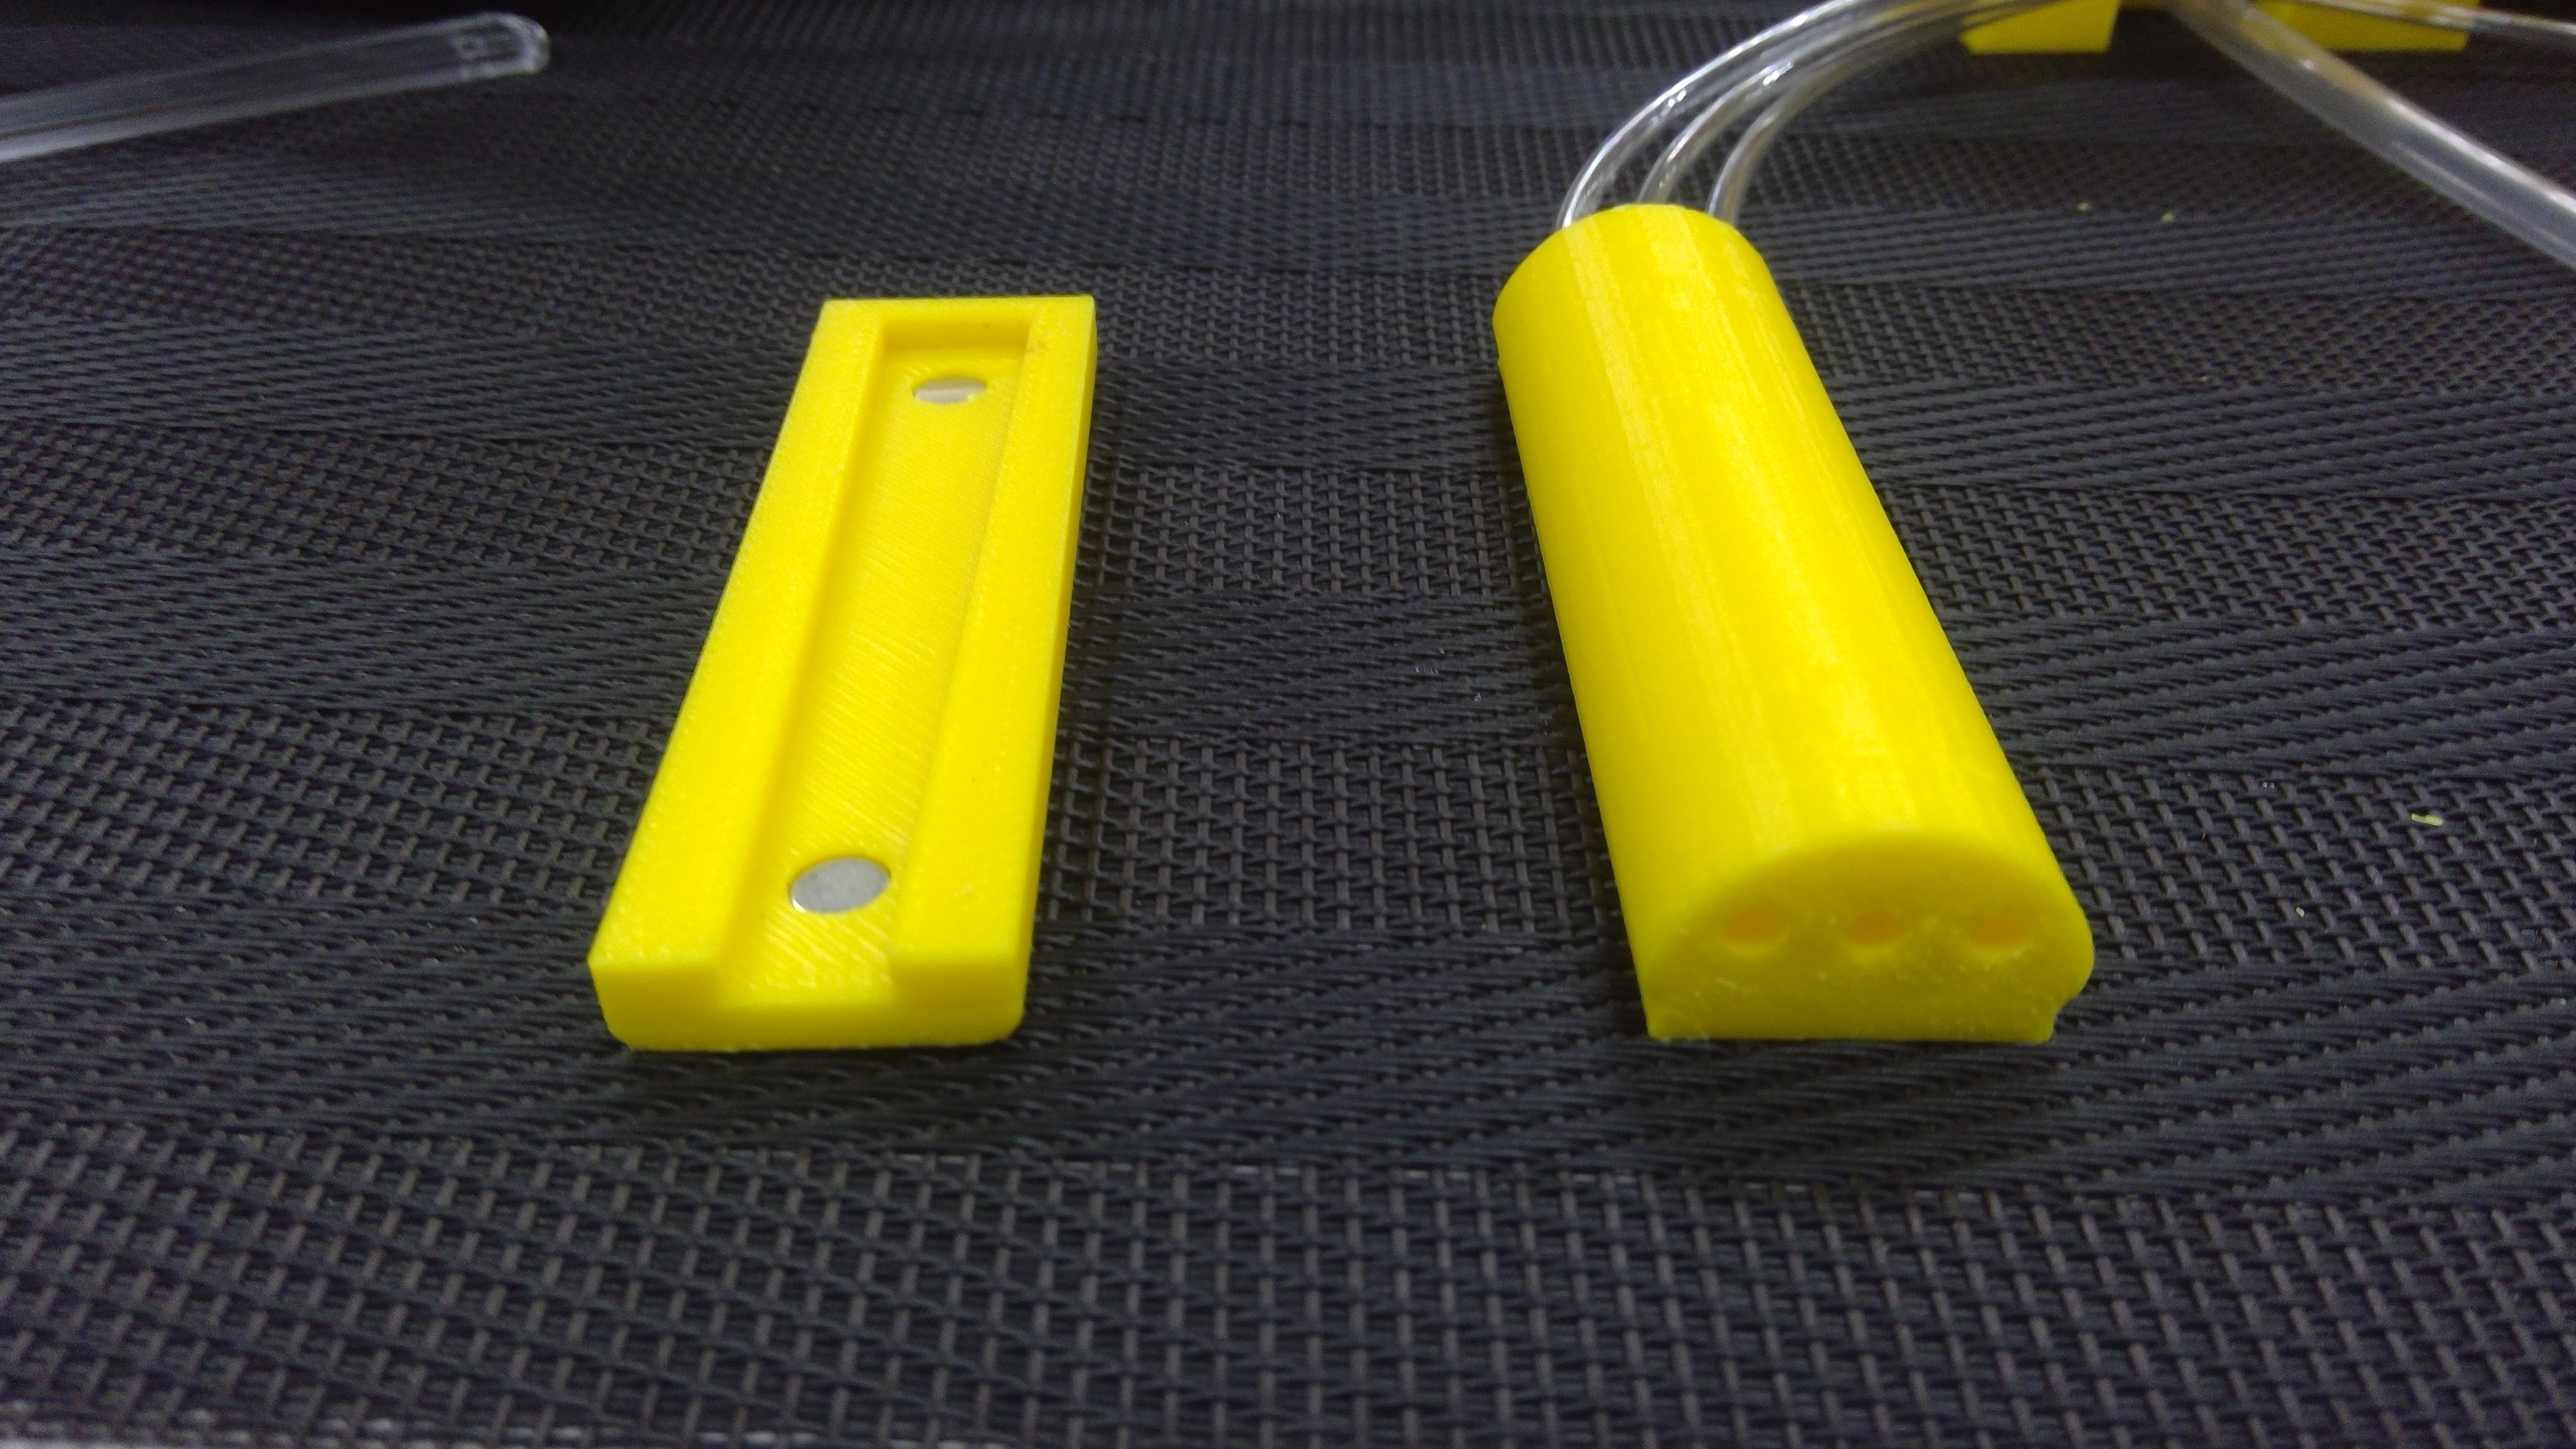
\includegraphics[width = 1.0\columnwidth]{supunpart.jpg}
  \includegraphics[width = 1.0\columnwidth]{supunbody.jpg}
  \caption{スプーンデバイス
  (上部・下部・全体)}
  \label{device}
\end{figure}
以前の研究では,ファンの大きさに合わせた四角柱の形をしており,持つことが非常に困難となっていた.そのために,手にフィットするちょうどよい大きさで作成している.
ボディは二つに分解することができ,これはスプーンの取り外しが簡単にすることができるようにするためである.上部のボディには香りを送るためにエアチューブを3本通している.そのうちの二つからは香りを含んだ風が流れ,残りは香りを含まない風を流す.下部のボディにはスプーンのサイズに合わせた溝を作っており,そこにスプーンをはめ込むことができる.かき氷を食べる食器は市販の透明なプラスチックスプーンを使用する.衛生面も考慮したうえで使い捨てのスプーンであることを重視し,ショットグラスのLEDの色が見えるように透明なスプーンを選択した.上部と下部のそれぞれボディに磁石を仕込むことで,二つのボディはくっつき安定する.この二つを組み合わせたボディをスプーンに取り付けることで口元にスプーンを運んだ時に,香りを含んだ風が鼻に当たる仕組みとなっている.




\subsubsection{香りの配送装置}
香りを配送する手段として,エアポンプによる風の配送で最終的にユーザーの鼻へと香りを届けている.風はゴムチューブを介して送られており,三又のエアー分岐管を経由することで,3つの経路に分けられる.分岐管には風の流れを制御するためにエアコックがついており,これにサーボモータを用いることで動きを制御する.図\ref{servo}のように,エアコックの上にサーボモータを設置し,二つを固定する.これによりArduinoで制御したサーボモータの動きと連動することでエアコックの開け閉めを可能とする.サーボモータの動きはタクトスイッチにより0度から90度の動きを指示し,これを香りを含ませる2つのチューブに対して実行する.
\begin{figure}[t]
  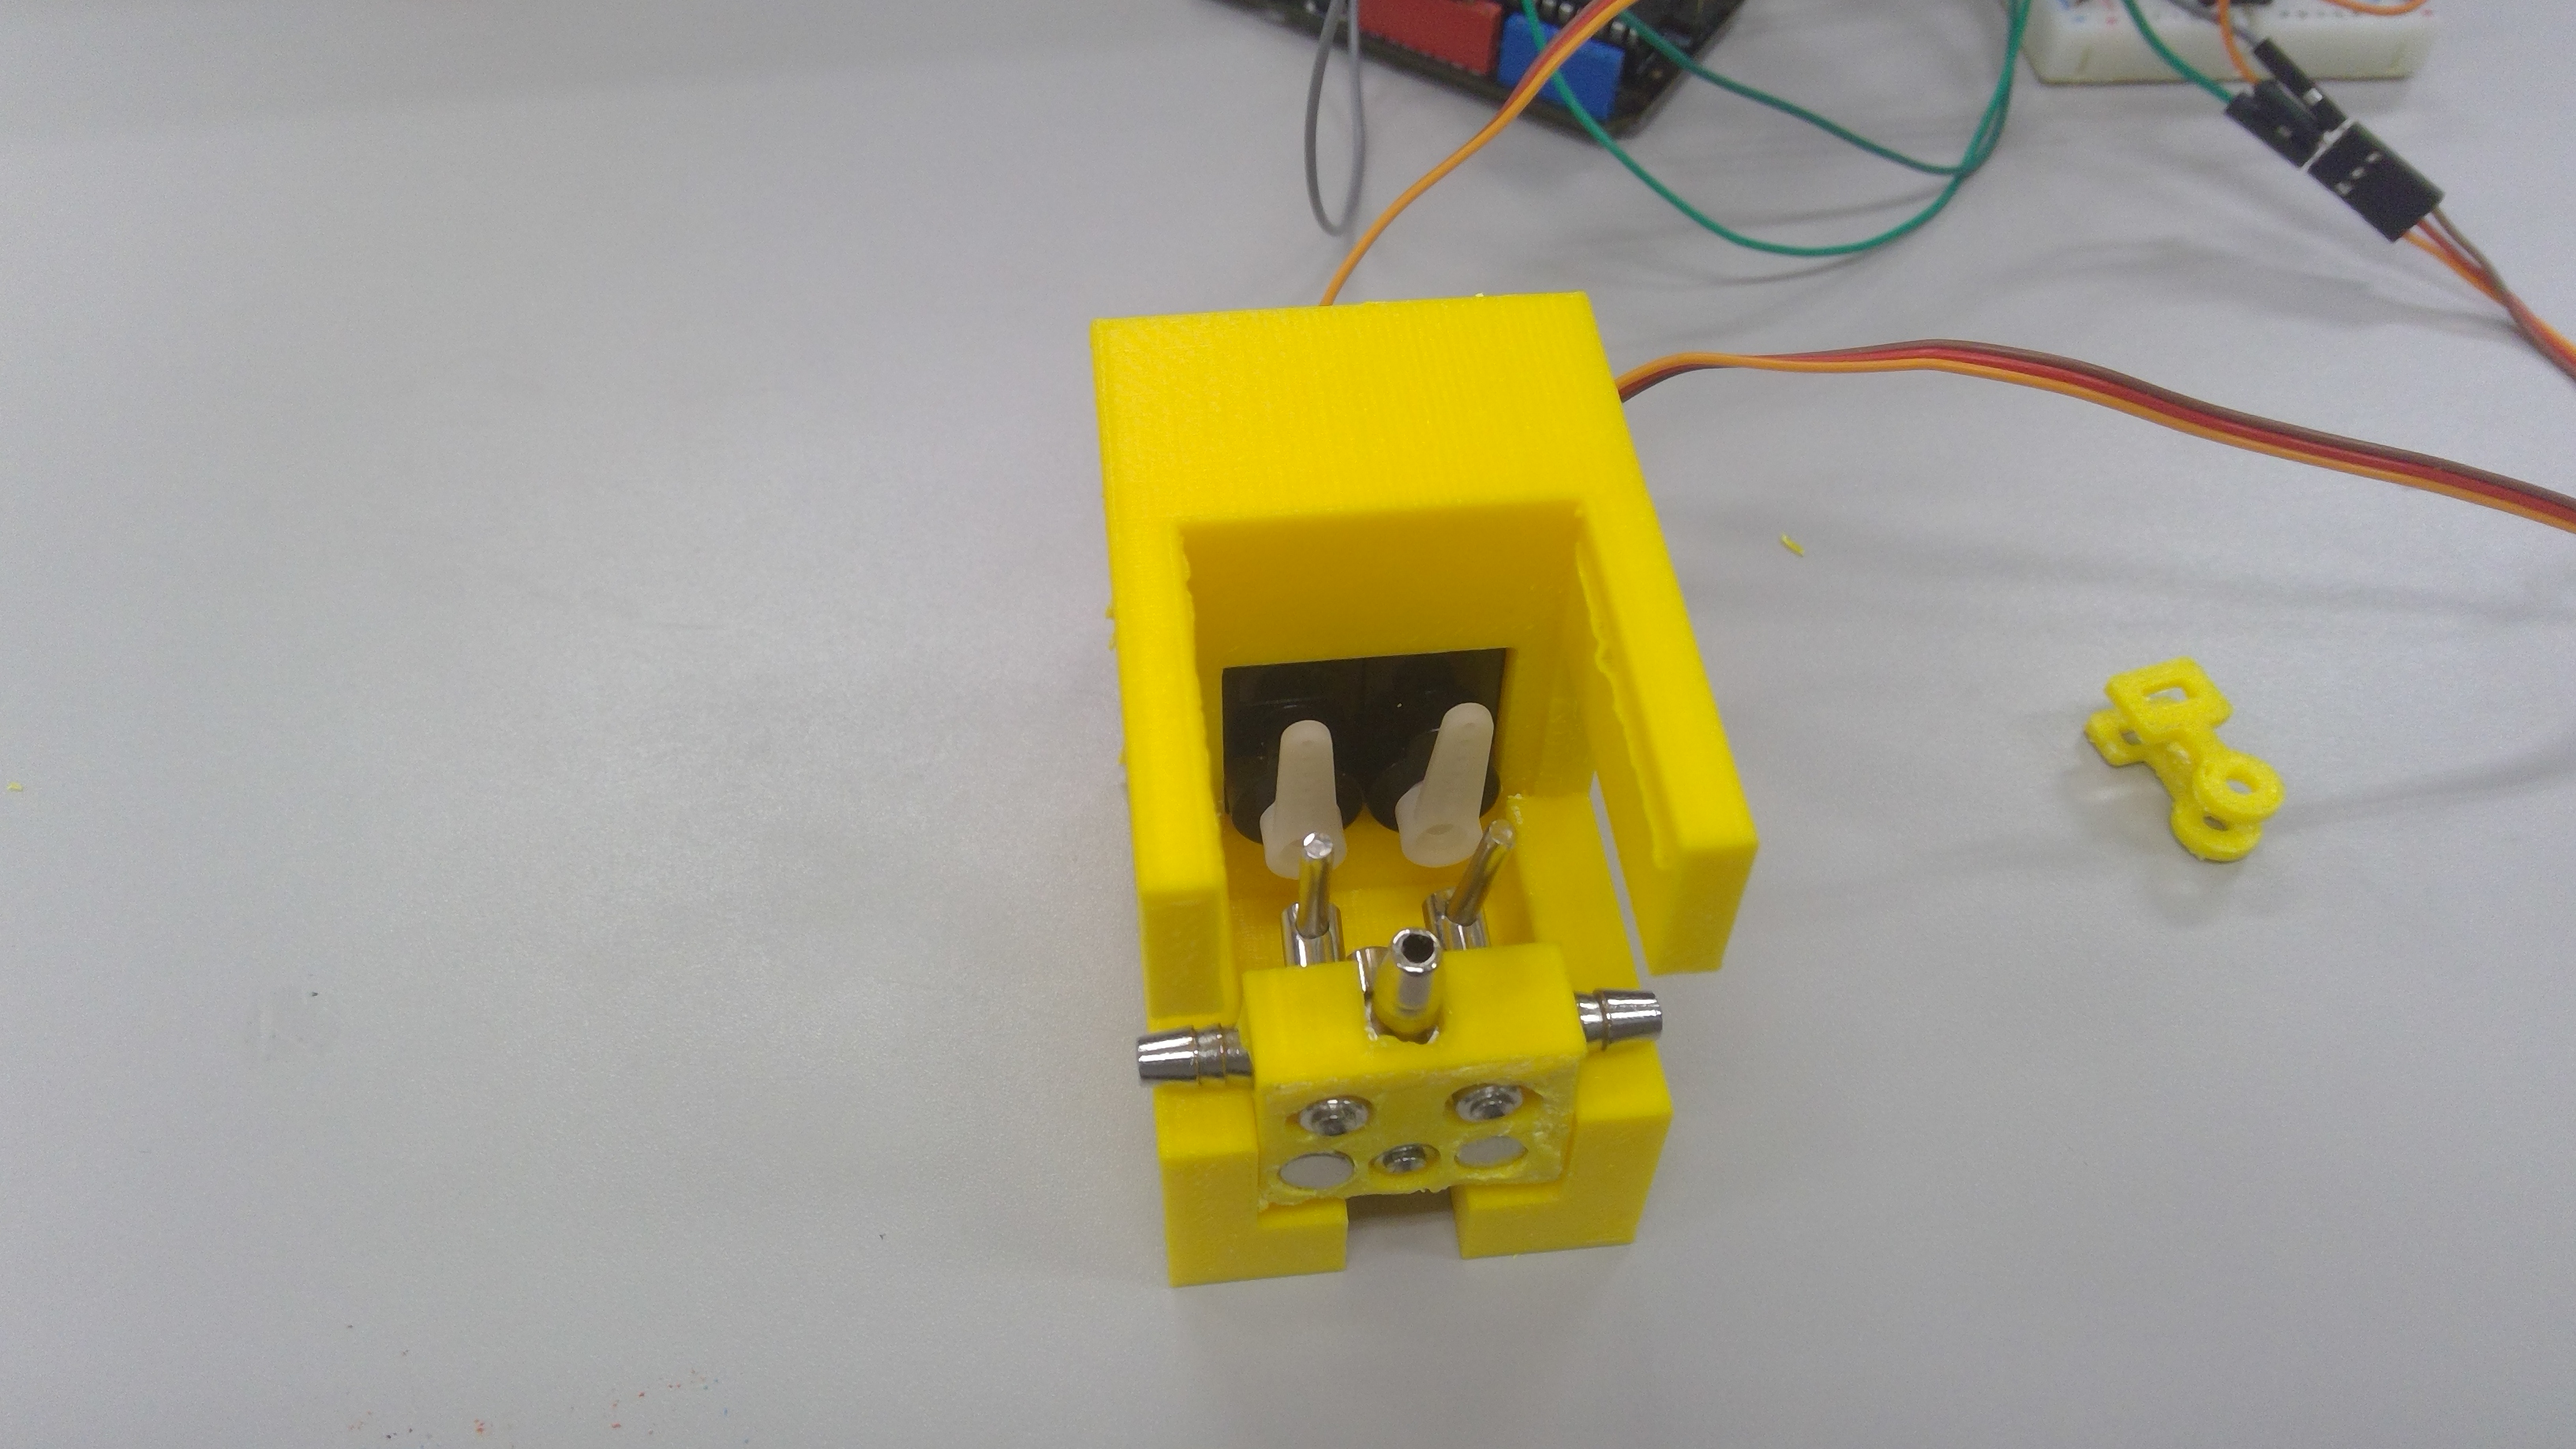
\includegraphics[width = 1.0\columnwidth]{servobox.jpg}
  \caption{サーボケースとエアー分岐管}
  \label{servo}
\end{figure}
この制御した風が流れる2つのチューブはそのまま図\ref{flavor}の香り瓶を経由することで香りを含ませることができる.前節で述べたように,今回はレモンとメロンの香りを用意しており,香り瓶の中にはこの二つの香りが仕込まれている.香り瓶の中には,香料を気化させやすくするために脱脂綿を入れる.香りを付与した風がそのままチューブを通じてスプーンデバイスへとつながる.残り1つのチューブでは何も含まない風を流し,制御せずにスプーンデバイスから流し続ける.これは香りを含んだ風を届ける際の補助となる風であり,配送していない際のスプーン周辺の換気のための風でもある.


\begin{figure}[t]
  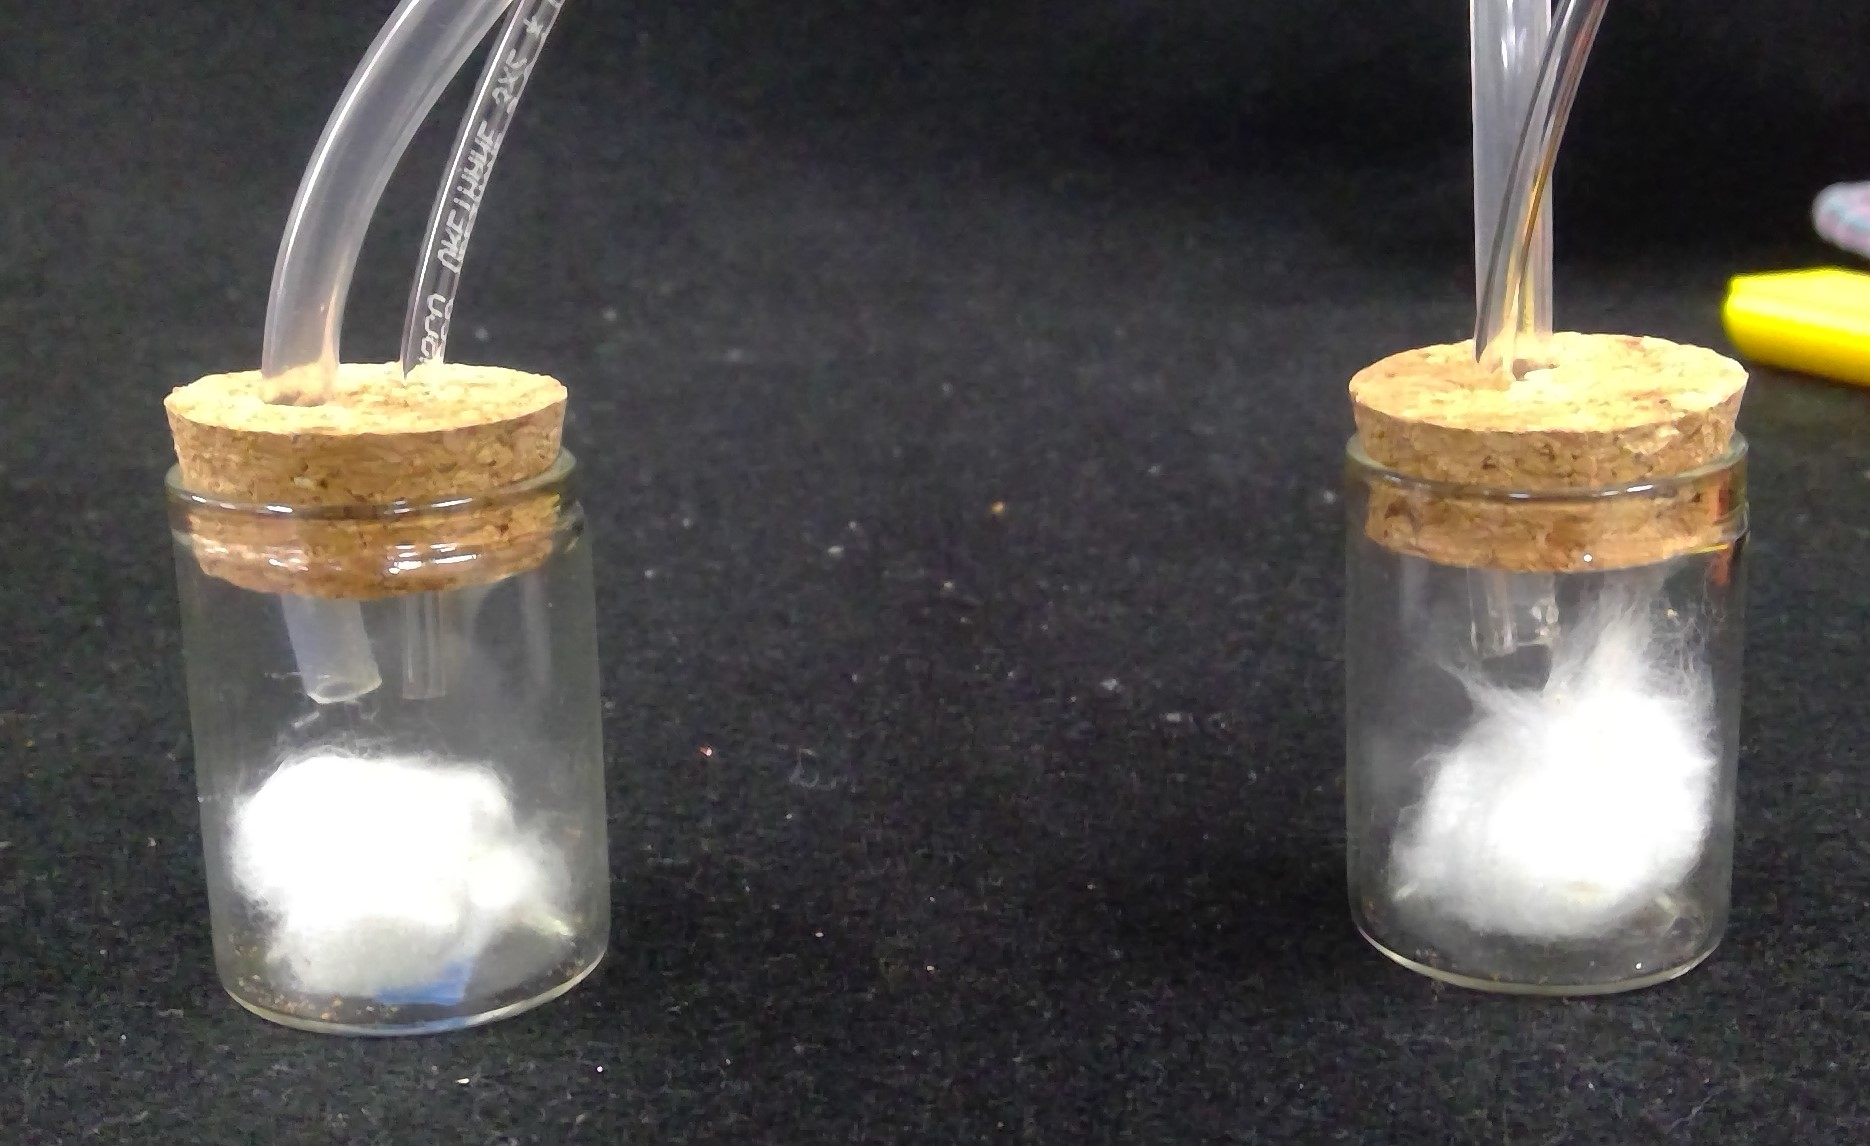
\includegraphics[width = 0.49\columnwidth]{flavorbin.jpg}
  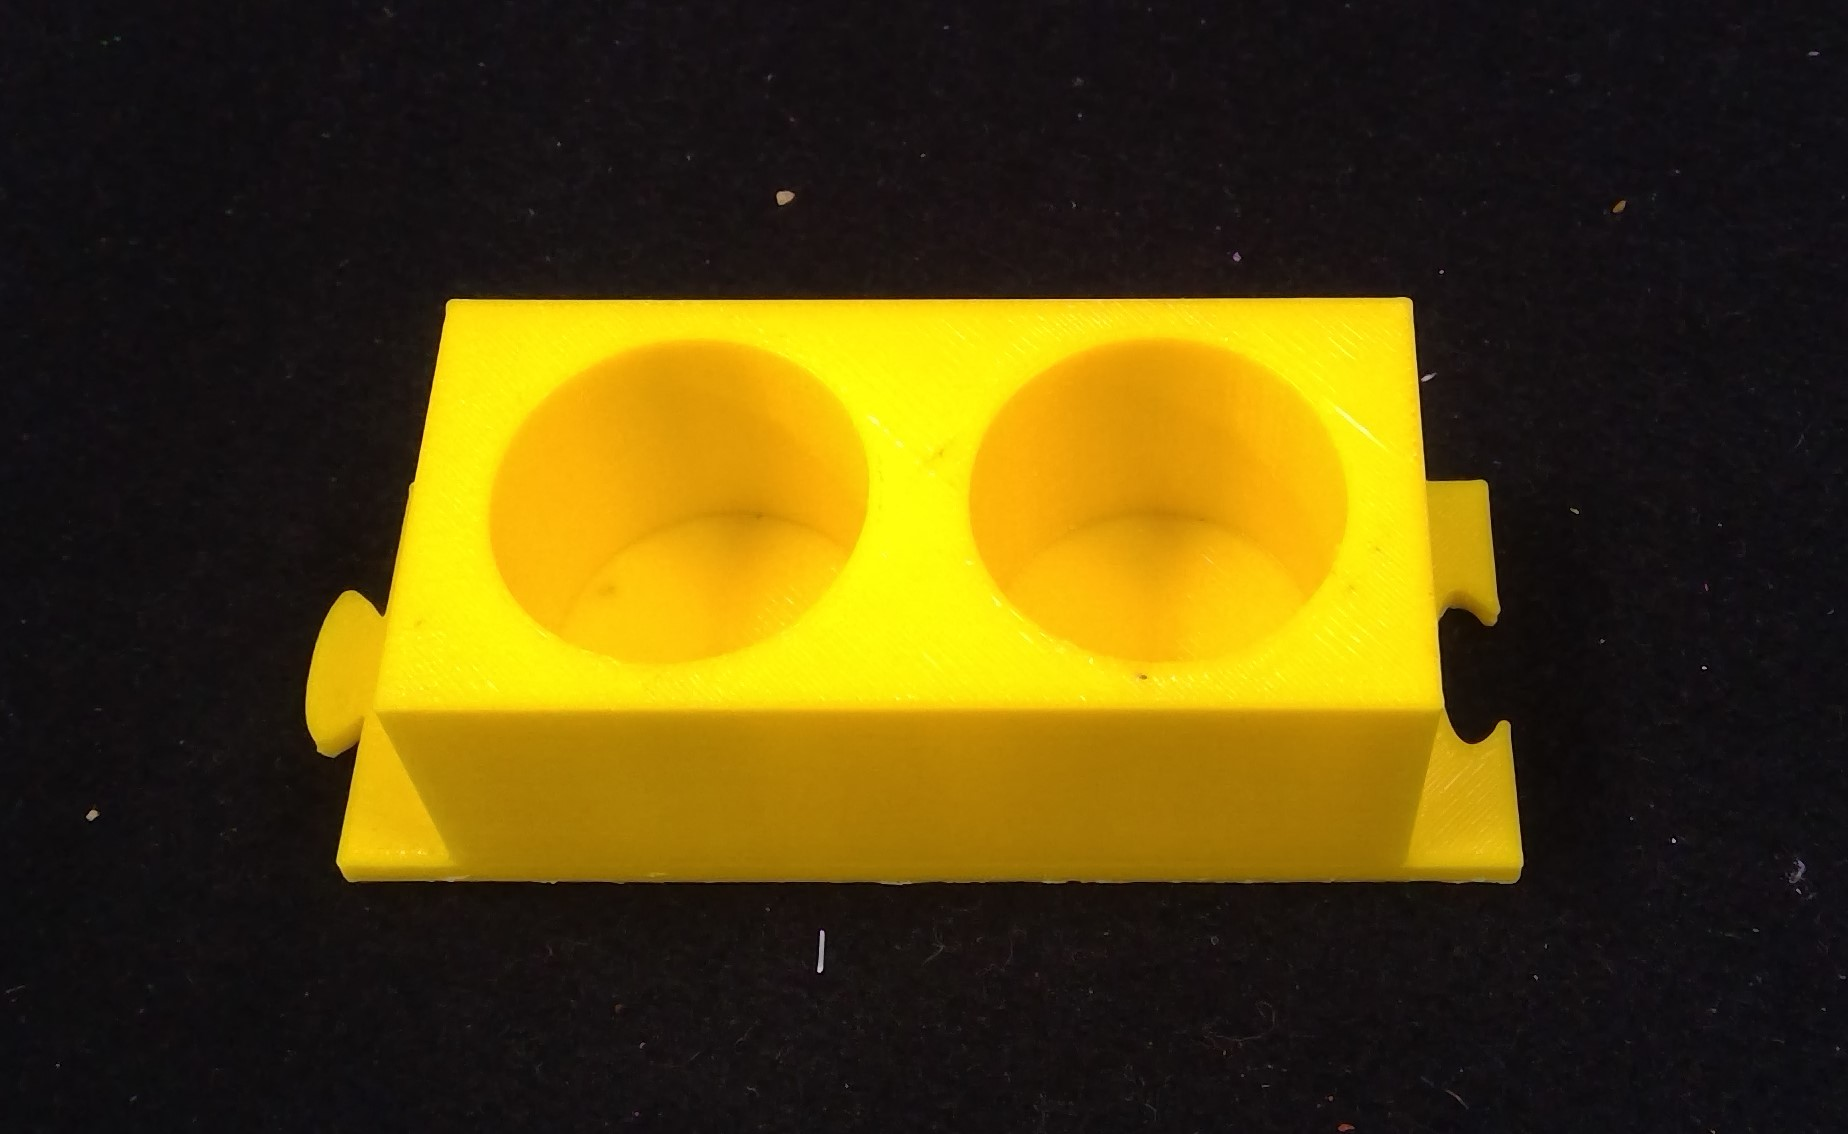
\includegraphics[width = 0.49\columnwidth]{bincase.jpg}
  %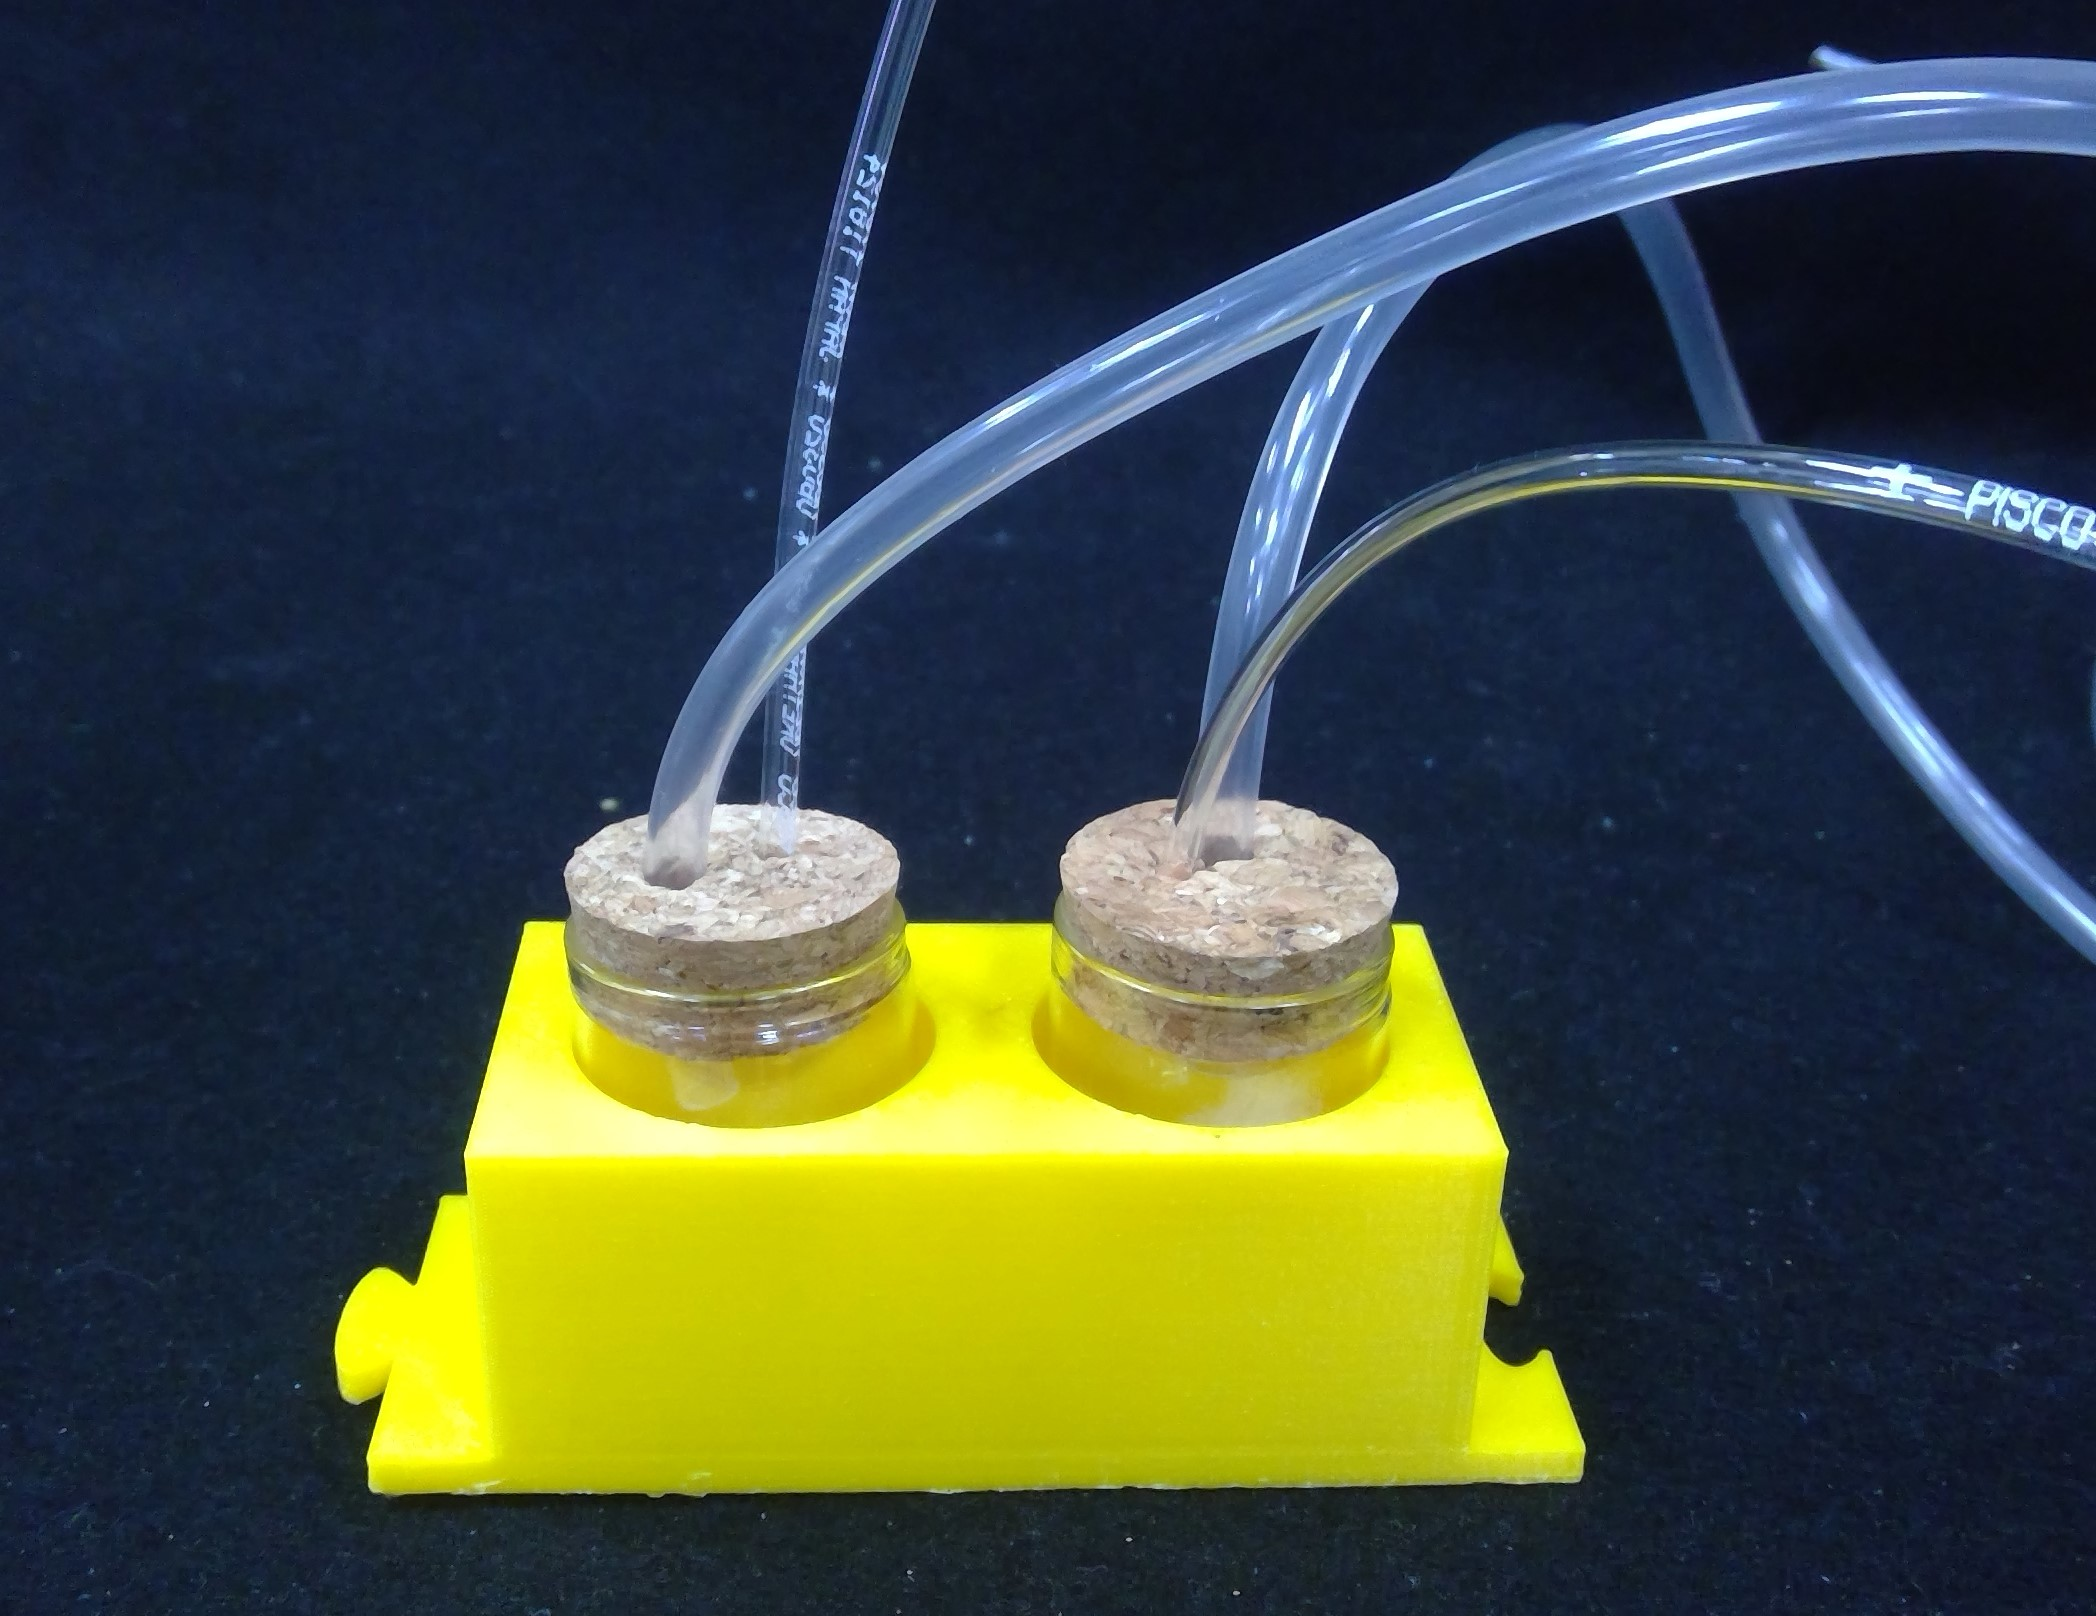
\includegraphics[scale = 0.075]{flavorcase.jpg}
  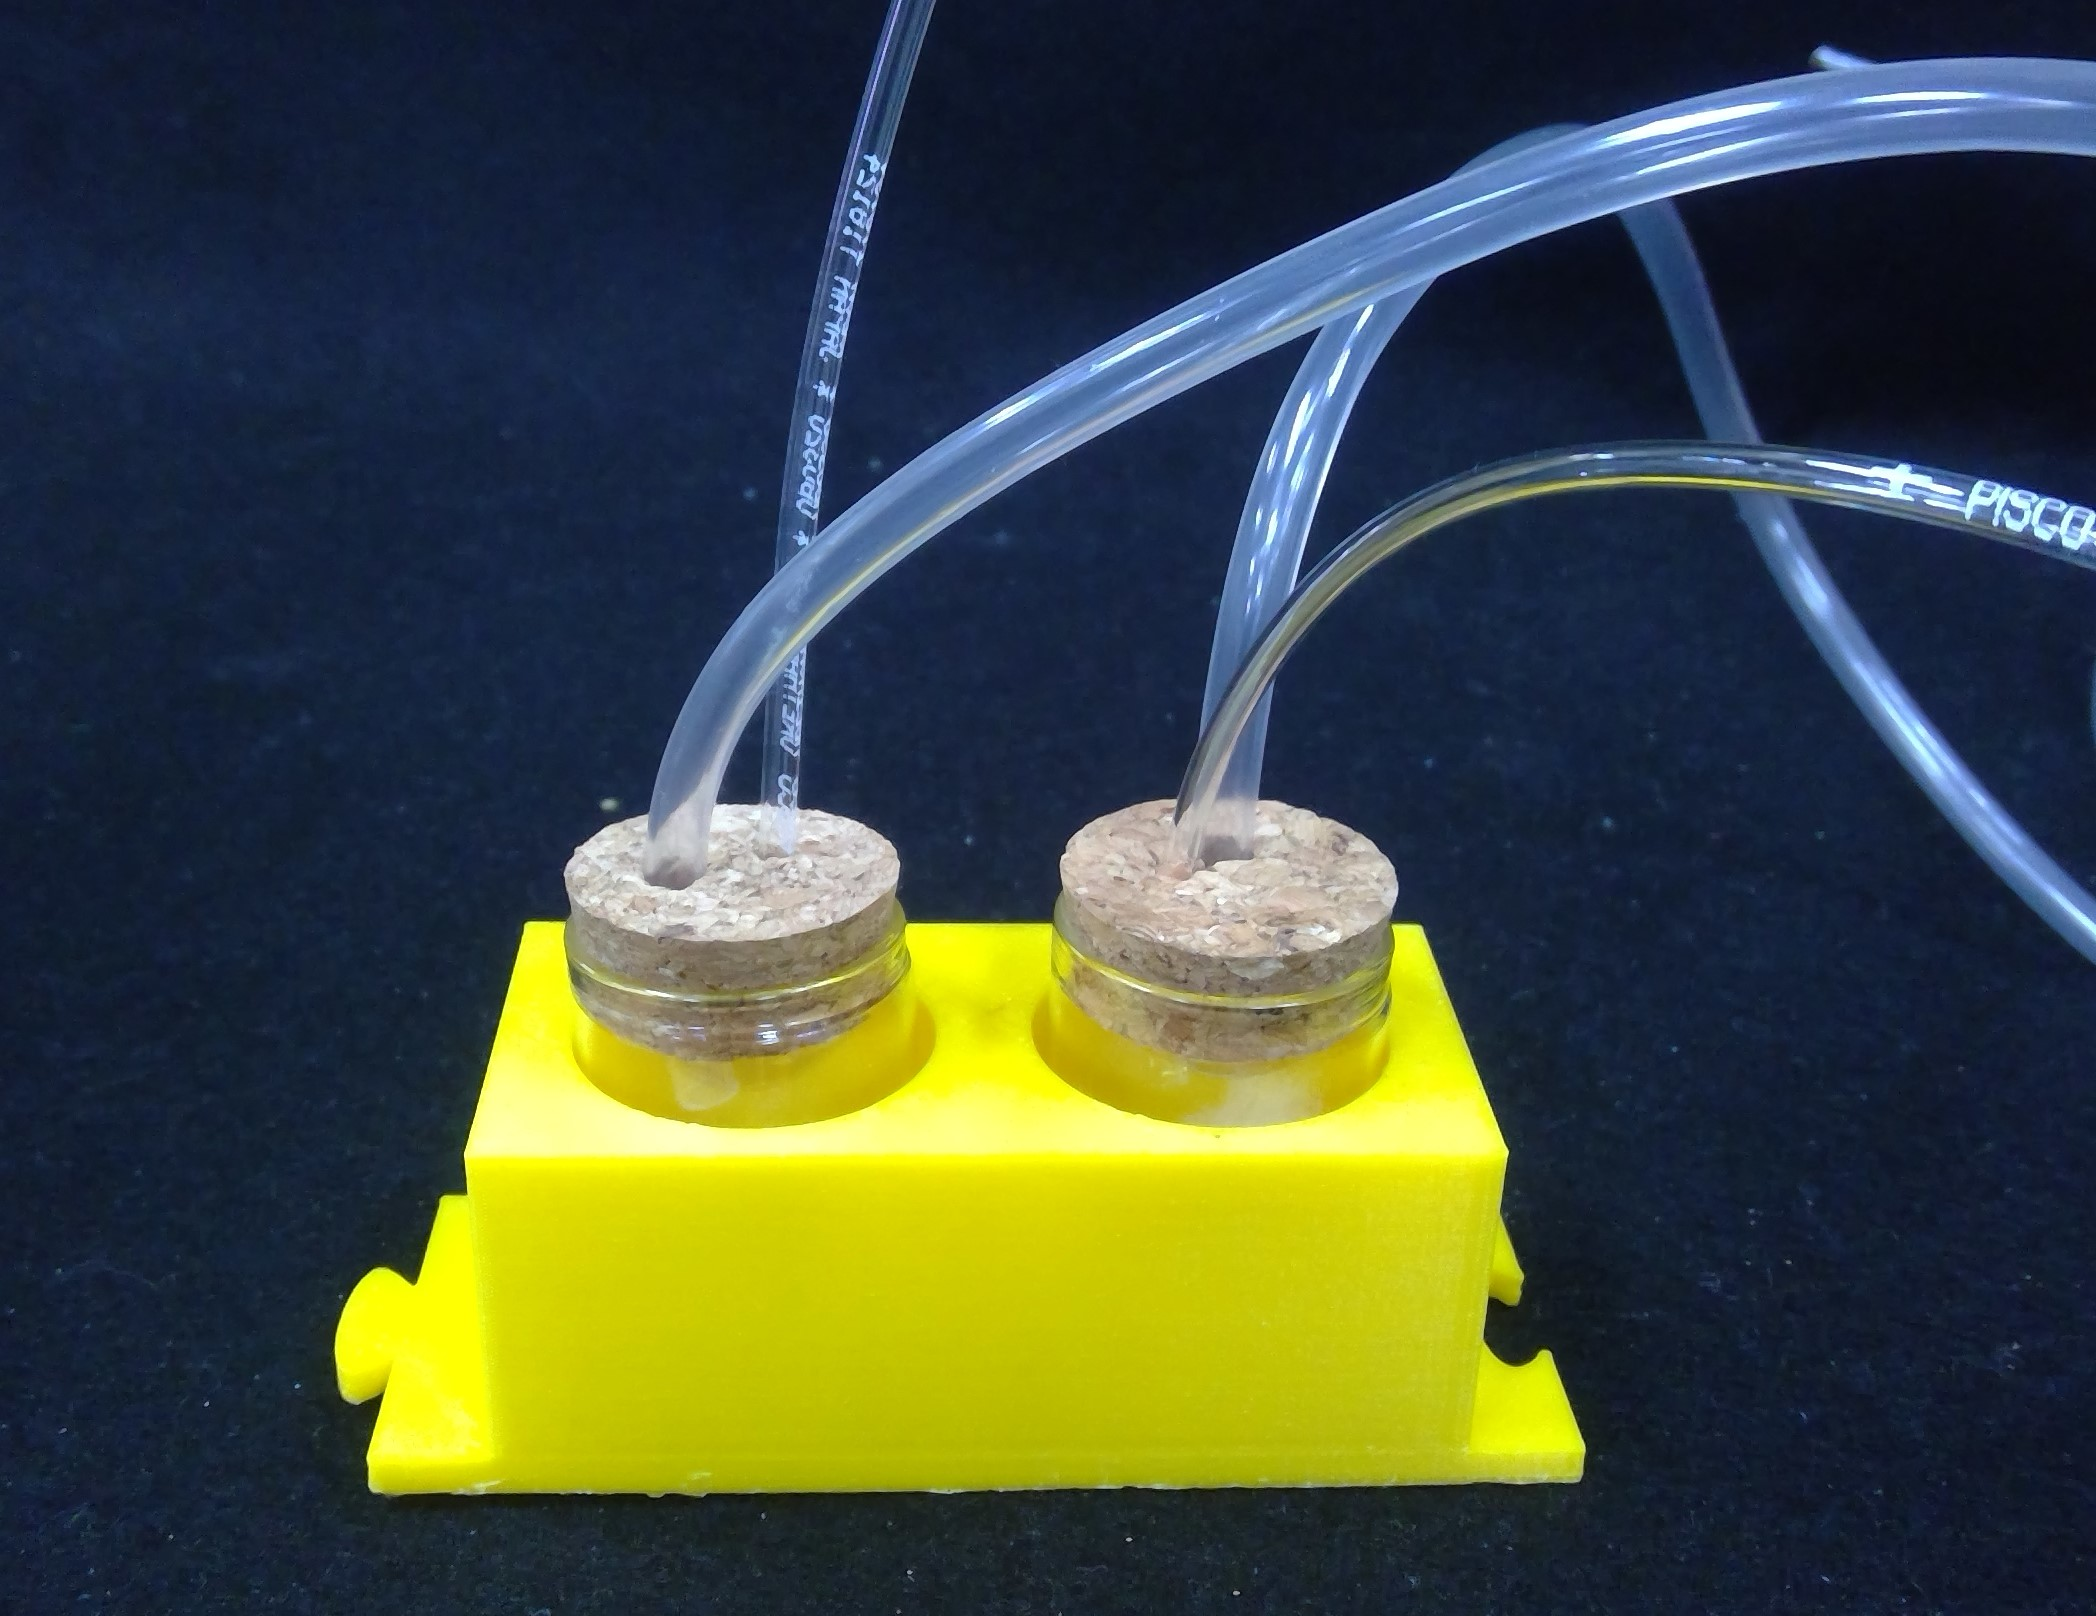
\includegraphics[width = 1.0\columnwidth]{flavorcase.jpg}
  \caption{香り瓶と香りボックス}
  \label{flavor}
\end{figure}


これらをまとめた嗅覚情報提示装置はリアルタイムのスムーズな香りの切り替えを可能とする.また,不必要な香りの漏洩を少なからず防ぎ,部屋に香りが充満することによる実験の弊害を多少なりとも防ぐことにつながる.

%5
\section{相互作用における味の提示実験}
% 目的
本実験では前述した手法を合わせることによる,リアルタイムに味を変化させる新たなデバイスを用いて,味覚に対して味を想起させることができるかを検討する.
スープの味には余計なものを感じさせない単純な塩味として塩とうま味成分を使用する.それに加え,香りをもたらすカップを使用することで味を想起させる.
今回の実験では,新たに作成した味覚変容デバイスの有用性を調査するとともに,新しく検証する塩味に対してアプローチがどの程度の認知を得るかを調査する実験である.

%3.4 全体の方法
\subsection{実験の方法}
まず実験を始める前に,直近で味のあるものをとったかどうかを確認し,目安30分以上開けて実験を遂行した.最初に,本実験では味の評価をしてもらう実験だと伝え,食べてもらうのは醤油と味噌の味であることを理解させた.

その後,評価用紙を提示し,それらを食べた経験があるかを問う.(この行程は考え中)この間に,実験者はスープの準備を行う.
スープはポットから用意するが,その作業風景は見せないようにした.
スープは・・・作り方,分量,中身の分量を記す・・・


そして,用意されたスープを作成したデバイスを用いて飲んでもらうように指示する.スープをのみ終わる,もしくは飲み終わりを宣言したら評価用紙に記入してもらい,その間にまた新しいスープを作成する.

この行程を2つの味+もとの味の3パターン行ってもらい,味の評価を4段階の評価(1:まったく感じない~4:すごく感じる)で変化の度合いを回答する.

%\begin{table}[tb]
%\caption{質問内容}
%\label{question}
%\hbox to\hsize{\hfil
%\begin{tabular}{l|lll}\hline\hline

%質問内容 & 評価 \\\hline
%香り:イチゴ(メロン)味 & 4段階評価\\\hline
%LED:イチゴ(メロン)味 & 4段階評価\\\hline
%香り+LED:イチゴ(メロン)味 & 4段階評価\\\hline
%\end{tabular}\hfil}
%\end{table}


なお,味の慣れや香りの混乱を避けるために一つの行程ごとに,被験者には評価用紙の記入してもらい,水で口を整えてもらう.実験者は容器を交換し新たなスープを用意することで時間を空けるようにした.
すべての味を食べた後には,食べてみたい味やコメントなどの自由意見を記入してもらうこととした.


本実験では,10代,20代の男女12名(男9名,女3名)に対しての調査を行った.

\begin{table}[tb]
\caption{質問内容}
\label{question}
\hbox to\hsize{\hfil
\begin{tabular}{l|lll}\hline\hline

質問内容 & 評価 \\\hline
醤油味だと感じましたか? & 4段階評価\\\hline
味噌味と感じましたか? & 4段階評価\\\hline
味だと感じましたか? & 4段階評価\\\hline
\end{tabular}\hfil}
\end{table}


%%4 結果と考察

\section{結果と考察}

\begin{figure}[t]
  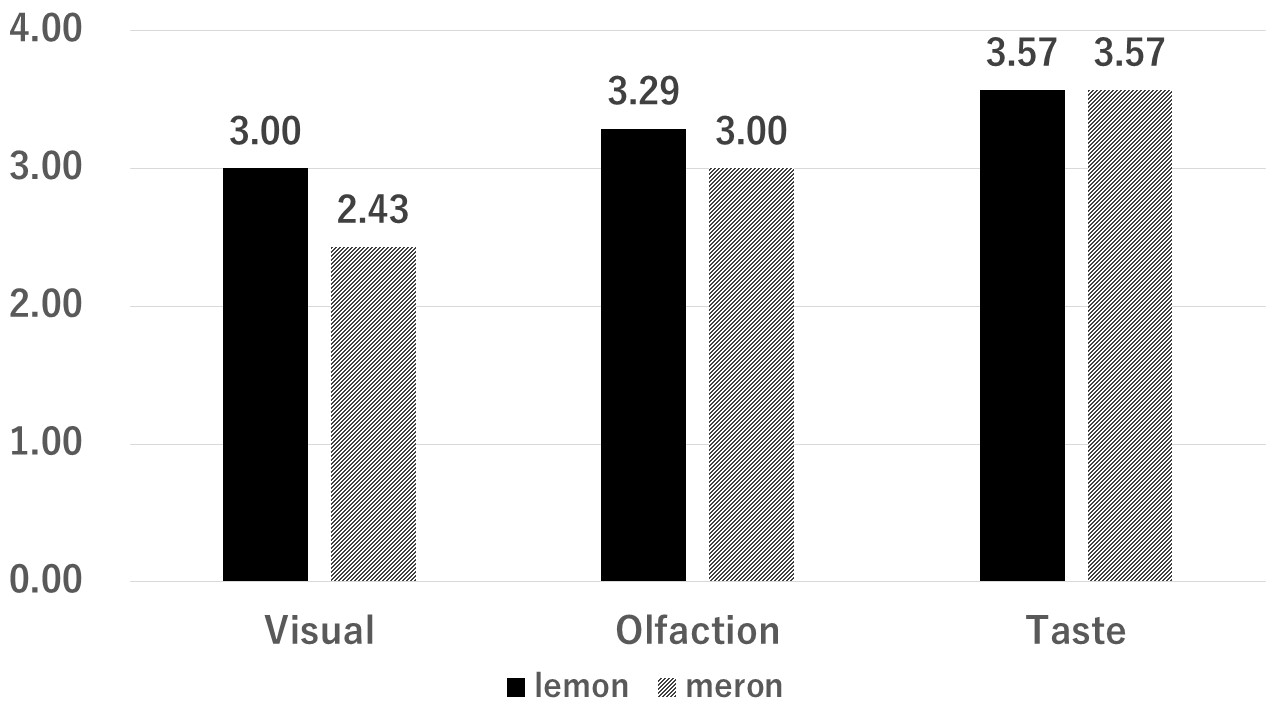
\includegraphics[width = 1.0\columnwidth]{figs/data.jpg}
  \caption{アンケートの平均スコア}
  \label{data}
\end{figure}
実験の結果を図\ref{data}に示す.


LEDで色を付けたかき氷の見た目における評価は,レモン味だと感じた平均スコアは3.00点,メロン味は2.43点であった.
これは前回の研究に引き続き,黄色がレモンの味であることを自然と印象付けている傾向にあることを示している.メロン味は半分を超えているが,印象としてはあまり良くなく,言われてみればわかるというものだった.
その一方で,「LEDによる色付けが,光っている印象が強く,色の違いが頭に入ってこなかった」という意見があった.このことから光量の強さも意識する必要がある.


嗅覚面における評価は,レモン味だと判断したのは3.29点,メロン味は3.00点であった.
どちらも評価としては高いが,意見の中で大きく違いが出た.レモン味は高い割合ではっきりとわかると答える一方で,メロン味は言われてみればという意見が多かった.自由記述にも,「あまり嗅いだことがない」,「ニオイがわかりづらい」といった記載があった.これは,メロンの香りを嗅ぎ慣れていないという体験の少なさが大きな原因となったと考えている.レモンのような柑橘系の香りは,食体験に限らず,消臭剤や芳香剤と言った身近なところにも溢れている.その一方でメロンの香りは体験することが少ないことから想起することができなかったと考えられる.


かき氷の味の感じ方の評価は,レモン味,メロン味共に3.57点と,その味を感じているという評価が多い結果となった.
レモン味は「一瞬レモンと感じたが,スプーンを離したとたんにすぐに甘い感じになった.レモンが打ち消された感覚だった」という意見から,以前の研究と同様に,一瞬の味を想起させるという目的では有効だが,しっかりと味を感じさせるという目的であれば違う手法が必要であると考える.
メロン味のほうでは.見た目と香りの評価が低いにもかかわらずメロン味の評価は高いものとなっている.
意見の中には「レモンよりもそれっぽかった」などといった,レモンに比べてポジティブなものが多かった.
その中において,メロン味のほうで,「後味がメロンの味がした」という意見を得られた.レモンとは逆で消えるのではなく残ったというのはとても興味深いものだった.甘い後味がメロンと類似するからではないかと考察する.

他にも「レモンの香りが強い」という記述が多く,ニオイの強さの制御に関しても考えていく必要がある.

%6
%
\section{おわりに}


本研究では,LEDとエアポンプを用いたリアルタイムに複数の味を体験できる味覚変容デバイスを開発した.
そして視覚情報と嗅覚情報の重畳を利用した一瞬の味覚の変化を起こす実験を行った.
新しいデバイスは,食べやすさがかなり改善され,そのような指摘を受けることはなかった.
香りの配送装置に関しても,単純な作業で香りの切り替えをスムーズに行うことができた.以前の研究で使用したファンと今回のエアポンプでは,空気の出る量や,鼻に風が当たる時の表面積の違いがあるが,ユーザーに対して香りをしっかりと感じてもらうことができていた.また多少の香りは出ていたものの,部屋の香りの充満をおさえることができていた.


このシステムは必要な分だけの香りを提供するためにコンパクトに作られている.
それによって一つの食べ物に対して複数の場所から出すことができると考えている.
具体的には,綿菓子のような表面積の広いものに対してニオイを出す場所を細かく配置することで,この場所は何味、他の場所は違う味と言ったような楽しみ方も可能性としてはあり,今後の検討にしていきたい.

現段階においては,香りは2種類までしか出せず,それ以上のものを試すためにはチューブをはめなおしたりしなければいけない.その点をうまく切り替える方法を考えなくてはいけない.

また,提示する香りの強度についての確認が必要である.
自由記述の中には,「レモンの香りが強い」という意見が2割程度見られ,口頭でもそのように回答するユーザーが多かった.
一つの香りの強さが印象に残り,ほかの香りの印象が残らないことで,味に対して影響を与えることは十分に考えられる.そのため香りの強度の制御やその影響の調査を行っていく必要がある.

今後の展望としては,香りの強度の適切な量の特定や,他の香りを試していくことでの味の変化を調査していくことが挙げられる.
その中で,複数の香りを混ぜることでまた味に対して何かしらの違いを生むことができるか調査したいと考えている.また,食べている段階で色と香りを切り替えることで,その場でも味の変化を感じるのかを検証したいと考えている.

以上で述べたことを実践していくことで,馴染みのない香りや色の刺激による組み合わせや香りを与える順番を変えることでの残り香による味の影響といった,バリエーションのある新しい食体験を感じてもらえるのではないかと考えている.



%このシステムを用いて,かき氷に対して色と香りを重畳し,その見た目・香り・味を評価してもらう実験を行った.その結果,味の変化を感じているという結果を得られ,狙った通りの味を認識させることができるという有効性を示した.

%この手法は,かき氷に限らずさまざまな食べ物に対して一瞬の味を想起させることができるのではないかと考えている.具体的には,砂糖菓子のような単純な甘さがあり無臭のものでなら行えるのではないかと考えており,今後の検討にしていきたい.

%現段階において,複数の香りを試す際に,そのたびにデバイスのボディを開き中の脱脂綿を入れ替えなければいけない.その手間をなくすための香り伝達の仕組みを考えなくてはいけない.
%また,提示する香りに関しての換気の重要性についてを改めて再確認した.今回の実験では被験者が入れ替わるごとに,窓を開きファンを回して換気を行っていた.
%しかしながら,時間がたつにつれて徐々に香りが部屋に充満していってしまった.このことにより被験者が余計な香りに気づいてしまうことがあった.
%加えて,使用する脱脂綿にも香りが互いに移りあい,混ざり合った香りとなっていた.
%そのため適宜交換のタイミングを見極める必要がある.

%今後の展望として,食べている段階で色と香りを切り替えることで,その場でも味の変化を感じるのかを検証したいと考えている.
%そのために,色だけ変えたもの,香りだけを与えたもの,両方を与えたものを比較実験としてより多くの対象に実践していくことが必要である.そして換気を行いやすくするための部屋を作ることを検討している.

%以上で述べたことを実践していくことで,さまざまなバリエーションのある味として認識させることができるのではないかと考えている.また馴染みのない香りや色の刺激といった組み合わせを試すことで新しい体験となるのではないかと考えている.


\bibliographystyle{ipsjunsrt}
\bibliography{src/bib}
%\begin{thebibliography}{10}

%\bibitem{latex}
%Lamport, L.: {\em A Document Preparation System \LaTeX User's Guide \&
%  Reference Manual}, Addison Wesley, Reading, Massachusetts (1986).
% (Cooke, E., et al.訳:文書処理システム \LaTeX,アスキー出版局
%  (1990)).

%\bibitem{total}
%伊藤和人: \LaTeX トータルガイド,秀和システムトレーディング (1991).
%\bibitem{nodera}
%野寺隆志:楽々 \LaTeX,共立出版 (1990).

\bibitem{okumura}
奥村晴彦:改訂第5版 \LaTeXe 美文書作成入門,
技術評論社(2010).

\bibitem{companion}
Goossens, M., Mittelbach, F. and Samarin, A.:
{\it The LaTeX Companion},
Addison Wesley, Reading, Massachusetts (1993).

\bibitem{book1}
木下是雄:
理科系の作文技術,
中公新書(1981).

\bibitem{book2}
Strunk W. J. and White E.B.:
{\it The Elements of Style, Forth Edition},
Longman (2000).

\bibitem{book3}
Blake G. and Bly R.W.:
{\it The Elements of Technical Writing},
Longman (1993).

\bibitem{book4}
Higham N.J.:
{\it Handbook of Writing for the Mathematical Sciences},
SIAM (1998).

\bibitem{webpage1}
情報処理学会論文誌ジャーナル編集委員会:
投稿者マニュアル(online),
\urlj{http://www.ipsj.or.jp/journal /submit/manual/j\_manual.html}
(2007.04.05).

\bibitem{webpage2}
情報処理学会論文誌ジャーナル編集委員会:
べからず集(online),
\urlj{http://www.ipsj.or.jp/journal/manual /bekarazu.html}
(2011.09.15).

\end{thebibliography}




%\appendix
%7
%\section{付録の書き方}

%付録がある場合には,参考文献リストの直後にコマンド \|\appendix| に引き続
%いて書く.付録では,\|\section| コマンドが{\bf A.1},{\bf A.2}などの見出
%しを生成する.

%7.1
%\subsection{見出しの例}

%付録の \|\subsetion| ではこのよう見出しになる.

%8
%\section{研究会論文用コマンド}
%\label{sig}

%各研究会論文誌(トランザクション)には各々に固有のサブタイトル,略称,通
%番がある.最終原稿では,以下のコマンドを \|\documentclass| の{\bf オプショ
%ン}とすることで,これらの情報を与える.

%\begin{itemize}
%\item \|PRO|(プログラミング)
%\item \|TOM|(数理モデル化と応用)
%\item \|TOD|(データベース)
%\item \|ACS|(コンピューティングシステム)
%\item \|CDS|(コンシューマ・デバイス\,\&\,システム)
%\item \|TBIO|(Bioinformatics)\footnote{%
%TBIO, SLDM, CVAは英文論文誌であるので和名はない.}
%\item \|SLDM|(System LSI Design Methodology)\footnotemark[5]
%\item \|CVA|(Computer Vision and Applicaitons)\footnotemark[5]
%\end{itemize}

%また英文論文作成の際には \|english| をオプションに追加すればよい.したがっ
%て,\|\documentclass[PRO]{ipsj}| とすれば「プログラミング」の和文用,
%\|\documentclass[PRO,english]| \|{ipsj}| とすれば英文用となる.

%また研究会には「号」と連動しない「発行月」があるため,学会あるいは編集委
%員会の指示に基づき,発行月を
%
%\begin{itemize}\item[]
%\|\setcounter{|{\bf 月数}\|}{<発行月>}|
%\end{itemize}
%
%によって指定する.

%この他,以下の各節で示すように,いくつかの論文誌に固有の機能を実現するた
%めのコマンドなどが用意されている.

%\newpage%%

%9
%\section{各分冊固有コマンド}

%各分冊によってそれぞれ細かい仕様が違うため,同じコマンドでも出力結果が異
%なる場合がある.また「再受付」,「再々受付」が入る場合があり,それらは

%\noindent
%和文では
%\begin{itemize}\item[]
%\|\|{\bf 再受付}\|{<年>}{<月>}{<日>}|\\
%\|\|{\bf 再再受付}\|{<年>}{<月>}{<日>}|
%\end{itemize}
%英文では
%\begin{itemize}\item[]
%\|\|{\bf rereceived}\|{<年>}{<月>}{<日>}|\\
%\|\|{\bf rerereceived}\|{<年>}{<月>}{<日>}|
%\end{itemize}
%とプリアンブルに追加する.

%9.1
%\subsection{\<「プログラミング(PRO)」固有機能}

%\<「論文誌:プログラミング」には論文以外に,プログラミング研究会での研究
%発表の内容梗概が含まれている.この内容梗概は,\|\documentclass|のオプショ
%ンとして\|abstract|を指定する.\ref{config}~節の\|\maketitle|までの内容
%からなるファイル(すなわち本文がないファイル)から生成する.なお\|\|{\bf
%受付}や\|\|{\bf 採録}は不要であるが,代わりに発表年月日を,

%\noindent
%和文では
%\begin{itemize}\item[]
%\|\|{\bf 発表}\|{<年>}{<月>}{<日>}|
%\end{itemize}
%英文では
%\begin{itemize}\item[]
%\|\|{\bf Presents}\|{<年>}{<月>}{<日>}|
%\end{itemize}
%により指定する.

%9.1
%\subsection{\<「データベース(TOD)」固有機能}

%\<「論文誌:データベース」の論文の担当編集委員は,
%\begin{itemize}\item[]
%\|\Editor{<氏名>}|
%\end{itemize}
%により指定する.和文では「担当編集委員」,英文では「Editor in Charge:」
%と入る.

%またスタイルの変更に伴い,\underline{本文の最後}に入るので,
%\|\end{document}|の前に直接置く.

%9.2
%\subsection{\<「コンシューマ・デバイス\,\&\,システム(CDS)」固有機能}

%\<「論文誌:コンシューマ・デバイス\,\&\,システム」では,
%論文の種類によって見出しが変わるため,
%オプションで切替えを行う.

%各種別は
%\begin{itemize}
%\item \|systems  |コンシューマ・システム論文\\
%\|         |Paper on Consumer Systems

%\item \|services |コンシューマ・サービス論文\\
%\|         |Paper on Consumer Services

%\item \|devices  |コンシューマ・デバイス論文\\
%\|         |Paper on Consumer Devices

%\item \|research |研究論文\\
%\|         |Research Paper
%\end{itemize}
%となる.

%和文のコンシューマ・システム論文なら,\\
%\|\documentclass[CDS,systems]{ipsj}|
%となり,英文原稿なら \|english|を追加すればよい.

%9.3
%\subsection{\<「Bioinformatics(TBIO)」固有機能}

%Trans.\ Bioinformatics (TBIO)は英文論文誌であるので,\|TBIO|オプションの
%指定によって自動的に\|english|オプションが指定されたものとみなされ,
%\|english| オプションの省略が可能.

%論文種別は以下の3種.
%\begin{itemize}
%\item \makebox[4.9zw][l]{指定なし} Original Paper (Default)
%\item \|Data     | Database/Software Paper
%\item \|Survey   | Survey Paper
%\end{itemize}

%\|\documentclass[TBIO]{ipsj}|でOriginal Paper,\\
%\|\documentclass[TBIO,Survey]{ipsj}|でSurvey Paperとなる.

%また,担当編集委員はTOD同様,\|\Editor|で定義するが,「Communicated by」
%となる.TOD同様,\|\end{document}|の前に直接置く.

%9.4
%\subsection{\<「Computer Vision and Applicaitons\\\<(CVA)」固有機能}

%Trans.\ CVAも英文論文誌であるため,\|english| オプションの省略が可.

%論文種別は3種類あり,
%\begin{itemize}
%\item \makebox[4.9zw][l]{指定なし} Regular Paper (Default)
%\item \|Research | Research Paper
%\item \|system   | Systems Paper
%\end{itemize}
%となる.

%TBIO同様,担当編集委員が入り,
%挿入文章もTBIO同様,「Communicated by」となる.

%9.5
%\subsection{\<「System LSI Design Methodology(SLDM)」固有機能}

%Trans.\ SLDMも英文論文誌であるため,\|english| オプションの省略が可.

%論文種別は2種類あり,
%\begin{itemize}
%\item \makebox[4.9zw][l]{指定なし} Regular Paper (Default)
%\item \|Short    | Short Paper
%\end{itemize}
%となる.

%SLDMも担当編集委員が入るが挿入文章が論文によって自動挿入文章が異なる.

%通常は「Recommended by Associate Editor:」,\|invited|のオプションが入っ
%た場合のみ,「Invited by Editor-in-Chief:」となる.



%% 以下は無視されます
\begin{biography}
\profile{m}{情報 太郎}{1970年生.1992年情報処理大学理学部情報科学科卒.
1994年同大大学院修士課程了.同年情報処理学会入社.オンライン出版の研究
に従事.電子情報通信学会,IEEE,ACM 各会員}
%
\profile{n}{処理 花子}{1960年生.1982年情報処理大学理学部情報科学科卒.
1984年同大大学院修士課程了.1987年同博士課程了.理学博士.1987年情報処
理大学助手.1992年架空大学助教授.1997年同大教授.オンライン出版の研究
に従事.2010年情報処理記念賞受賞.電子情報通信学会,IEEE,IEEE-CS,ACM
各会員}
%
\profile{s}{学会 次郎}{1950年生.1974年架空大学大学院修士課程了.
1987年同博士課程了.工学博士.1977年架空大学助手.1992年情報処理大学助
教授.1987年同大教授.2000年から情報処理学会顧問.オンライン出版の研究
に従事.2010年情報処理記念賞受賞.情報処理学会理事.電子情報通信学会,
IEEE,IEEE-CS,ACM 各会員}
%
\end{biography}



\end{document}
